\chapter{Orientation Parametrization} \label{chap:appen-orientparam}

This appendix chapter will explore different orientation parametrizations. For completeness the sections in the report on quaternions and rotation matrices are added.

%TODO their advantages; and disadvantages. 

\section{Rotation Vectors}
\label{sec:rotation_vector}
It is possible to express the rotation between two coordinate systems as an angle ($\alpha$) and a unit vector ($n$) around which the rotation occurs, as

\begin{equation}
	\label{eq:rot_vec_rela}
	x^{\mathrm{u}}=x^{\mathrm{v}} \cos \alpha+n\left(x^{\mathrm{v}} \cdot n\right)(1-\cos \alpha)-\left(n\times x^{\mathrm{v}}\right) \sin \alpha
\end{equation}

where the superscripts indicate coordinate systems, thus indicating how vector $x$ in frame $v$ is expressed in frame $u$. The combination of $n$ and $\alpha$, 

\begin{equation}
	\label{eq:rotation_vector}
	\eta = n \alpha,
\end{equation}

is known as the rotation vector or axis-angle parametrization \cite{Kok2017}.



\section{Rotation Matrices}
Rotation matrices $R \in \mathbb{R}^{3 \times 3}$ have the following properties:

\begin{equation}
	\label{eq:app_rot_mat_properties}
	R R^{\top}=R^{\top} R=I_{3}, \quad \text { det } R=1.
\end{equation}

These matrices can be used to express a vector $x$ in frame $v$ to frame $u$ as 

\begin{equation}
	\label{eq:app_rot_mat_rot_x}
	x^{\mathfrak{u}}=R^{\mathfrak{u} \mathrm{v}} x^{\mathrm{v}}.
\end{equation}

Transposing a rotation matrix represent a rotation back to it's experimental coordinate frame:
\begin{subequations}
	\begin{align}
		\label{eq:app_rot_mat_trans}
		x^{\mathrm{v}}&=\left(R^{\mathrm{uv}}\right)^{\top} x^{\mathrm{u}},\\
		&=R^{\mathrm{vu}} x^{\mathrm{u}}.
	\end{align}
\end{subequations}

\section{Euler Angles}
Euler angles define a rotation as consecutive rotations around three axis using rotation matrices. These three rotations are know as yaw $ \phi $, pitch $ \theta $ and roll $ \psi $ representing a rotation around the $ z,y $ and $ x $ axis, respectively. A rotation defined through euler angles is represented by 

\begin{align}	
	R^{bn} &=R^{bn}(\phi) R^{bn}(\theta) R^{bn}(\psi) \\
	R^{bn} &=
	\left[\begin{array}{ccc}
			1 & 0 & 0 \\
			0 & \cos (\phi) & \sin (\phi) \\
			0 & -\sin (\phi) & \cos (\phi)
		\end{array}\right]
	\left[\begin{array}{ccc}
			\cos (\theta) & 0 & -\sin (\theta) \\
			0 & 1 & 0 \\
			\sin (\theta) & 0 & \cos (\theta)
		\end{array}\right] 
	\left[\begin{array}{ccc}
			\cos (\psi) & \sin (\psi) & 0 \\
			-\sin (\psi) & \cos (\psi) & 0 \\
			0 & 0 & 1
		\end{array}\right] \\
	R^{bn} &= \left[\begin{array}{ccc}
		\cos (\theta) \cos (\psi) & \cos (\theta) \sin (\psi) & -\sin (\theta) \\
		\sin (\phi) \sin (\theta) \cos (\psi)-\cos (\phi) \sin (\psi) & \sin (\phi) \sin (\theta) \sin (\psi)+\cos (\phi) \cos (\psi) & \sin (\phi) \cos (\theta) \\
		\cos (\phi) \sin (\theta) \cos (\psi)+\sin (\phi) \sin (\psi) & \cos (\phi) \sin (\theta) \sin (\psi)-\sin (\phi) \cos (\psi) & \cos (\phi) \cos (\theta)
	\end{array}\right].
\end{align}

A limitation of Euler angle representations is that they are not unique descriptions of a rotation, caused by \textit{wrapping} of the Euler angles. This causes  the rotation $ (0, 0, 0) $ to be equal to the rotation $ (0, 0, 2\pi k) $ for any integer $ k $ \cite{Kok2017}.\par 

Another limitation is a phenomenon known as \textit{gimbal lock}. This is where one degree of freedom is lost due to two rotations ending up causing rotations in the same dimensional plane \cite{Kok2017}.\par 

One of the large advantages of euler angles is that they are more intuitive to interpret than many of the other orientation parametrizations.


\section{Quaternions}
\label{sec:app_quaternion}
A quarternion is a common parametrization of orientation frequently used by attitude estimation algorithms. A unit quaternion can be described by

\begin{equation}
	\label{eq:app_unit_quarternion}
	q=\left(\begin{array}{llll}{q_{0}} & {q_{1}} & {q_{2}} & {q_{3}}\end{array}\right)^{\top}
	=\left(\begin{array}{l}{q_{0}} \\ {q_{v}}\end{array}\right), 
	\quad q \in \mathbb{R}^{4}, 
	\quad\|q\|_{2}=1.
\end{equation}

A rotation of vector $x$ using quaternions between two frames, from $v$ to $u$, is indicated as

\begin{equation}
	\label{eq:app_quat_rot}
	\bar{x}^{\mathrm{u}}=q^{\mathrm{uv}} \odot \bar{x}^{\mathrm{v}} \odot q^{\mathrm{vu}},
\end{equation}

where $q^{\mathrm{vu}} = \left(q^{\mathrm{uv}}\right)^{\mathrm{c}}$, with the latter representing the quaternion conjugate, defined by 

\begin{equation}
	\label{eq:app_quat_conjugate}
	q^{\mathrm{c}}=\left(\begin{array}{c}{q_{0}} \\ {-q_{v}}\end{array}\right).
\end{equation}

$\bar{x}^u$ represents the quaternion version of the vector $x^u \in \mathbb{R}^3$, as

\begin{equation}
	\label{eq:app_quat_vec_ref}
	\bar{x}^u=\left(\begin{array}{l}{0} \\ {x^u}\end{array}\right).
\end{equation}


The $\odot$ operator describes quaternion multiplication, defined by:

\begin{equation}
	\label{eq:app_quat_multiplication}
	p \odot q=\left(\begin{array}{c}{p_{0} q_{0}-p_{v} \cdot q_{v}} \\ {p_{0} q_{v}+q_{0} p_{v}+p_{v} \times q_{v}}\end{array}\right)
\end{equation}

It is also possible to define an orientation in terms of a linearization point and an orientation deviation using a rotation vector $\eta$. This is indicated as 
\begin{equation}
	q_{t}^{\mathrm{nb}} = \exp _{\mathrm{q}}\left(\frac{\eta_{t}^{\mathrm{n}}}{2}\right) \odot \tilde{q}_{t}^{\mathrm{nb}} \label{eq:quat_linear},
\end{equation}

where $\tilde{q}$ is a unit quaternion and $\exp_\mathrm{q}$ \cite{Kok2017} is defined as

\begin{equation}
	\exp_\mathrm{q} (\bar{\eta}) = \left(\begin{array}{c}{\cos \|\eta\|_{2}} \\ {\frac{\eta}{\|\eta\|_{2}} \sin \|\eta\|_{2}}\end{array}\right) \label{eq:exp_q}.
\end{equation}



\section{Orientation Parametrization Mappings}
Since all orientation parametrizations essentially represent the same phenomenon, all of them can be written from one to another. These translations are frequently used within the different \ac{PDR} methods. This section will outline the different mappings from each of the above parametrizations to the others.

\subsection{Rotation Matrix Mappings}
\label{sec:rotmatmappings}

The mapping from rotation vector to rotation matrix, with the definitions of $n$ and $\alpha$ indicated in \secref{sec:rotation_vector}, is

\begin{subequations}
	\begin{align}
		\label{eq:rotvec2rotmat}
		R\left(n, \alpha\right) &=\mathcal{I}_{3}-\sin \alpha\left[n \times\right]+(1-\cos \alpha)\left[n \times\right]^{2} \\
		& =\exp \left(-\alpha\left[n \times\right]\right),
	\end{align}
\end{subequations}


the derivation of which can be found in \citet{Kok2017}.

Note here that $\left[\mathrm{u} \times\right]$ represents how  a cross product can be written as a matrix vector product. It transforms a vector into a skew symmetric matrix, as shown:

\begin{equation}
	\label{eq:app_veccrossprod}
	u \times v=[u \times] v=-[v \times] u, \quad[u \times] \triangleq\left(\begin{array}{ccc}{0} & {-u_{3}} & {u_{2}} \\ {u_{3}} & {0} & {-u_{1}} \\ {-u_{2}} & {u_{1}} & {0}\end{array}\right).
\end{equation}

The inverse operation, from skew symmetric matrix to vector is indicated with $\operatorname{vex}$, defined as
\begin{equation}
	\label{eq:app_invveccrossprod}
	\operatorname{vex}([v \times]) = v
\end{equation}

The mapping from quaternion to rotation matrix is

\begin{equation}
	\label{eqapp_:quat2rotmat}
	R(q) = q_{v} q_{v}^{\top}+q_{0}^{2} \mathcal{I}_{3}+2 q_{0}\left[q_{v} \times\right]+\left[q_{v} \times\right]^{2}.
\end{equation}

Where $q$ with subscript uses the definition defined in \eqref{eq:app_unit_quarternion}.


\subsection{Rotation Vector Mappings}
The mapping from rotation matrix to rotation vector is 

\begin{subequations}
	\begin{align}
		\label{eq:app_rotmat2rotvec}
		\alpha &= \cos ^{-1}\left(\frac{1}{2}(\operatorname{Tr}\{R\}-1)\right),
		\\
		u &= \frac{1}{\sin (\alpha)} \operatorname{vex}\left(\frac{1}{2}\left(R-R^{\top}\right)\right).
	\end{align}
\end{subequations}


%TODO: how to cite equations now \cite{Hashim2019}.

Where $\operatorname{Tr}$ represents the trace of the $R \in \mathbb{R}^{3 \times 3}$ matrix. The operator $\operatorname{vex}$ is defined in \eqref{eq:app_invveccrossprod}.\\
The mapping from quaternion to rotation vector is 
\begin{subequations}
	\begin{align}
		\label{eq:quat2rotvec}
		\alpha &=2 \cos ^{-1}\left(q_{0}\right) \\ 
		u &=\frac{1}{\sin (\alpha / 2)} q_v 
	\end{align}
\end{subequations}


Where $q$ with subscript uses the definition defined in \eqref{eq:app_unit_quarternion}.

\subsection{Quaternion Mappings}

The mapping from rotation matrix to quaternion is %\cite{Hashim2019}. 

\begin{equation}
	\label{eq:app_rotmat2quat}
	\begin{aligned} q_{0} &=\frac{1}{2} \sqrt{1+R_{(1,1)}+R_{(2,2)}+R_{(3,3)}} \\ 
		q_{1} &=\frac{1}{4 q_{0}}\left(R_{(3,2)}-R_{(2,3)}\right) \\ 
		q_{2} &=\frac{1}{4 q_{0}}\left(R_{(1,3)}-R_{(3,1)}\right) \\ 
		q_{3} &=\frac{1}{4 q_{0}}\left(R_{(2,1)}-R_{(1,2)}\right) \end{aligned}
\end{equation}

Here the subscript on $R$ refers to the index of the $R \in \mathbb{R}^{3 \times 3}$ matrix component, while subscript on $q$ follows the definition of \eqref{eq:app_unit_quarternion}. \\
The mapping from rotation vector to quaternion is %\cite{Hashim2019}.

\begin{equation}
	\label{eq:app_rotvec2quat}
	q =\left[\begin{array}{l}{\cos (\alpha / 2)} \\
		{n \sin (\alpha / 2)} \end{array}\right].
\end{equation}

\chapter{Indoor Localization Experiment}
\label{appendix:shs_experiment}
\textbf{Apparatus}:

\emph{Hardware}:

\begin{itemize}
	\item
	3 Smartphones
	
	\begin{itemize}
		\tightlist
		\item
		Samsung j5 for video recording
		\item
		Iphone for backup orientation estimation and post processing time
		synchronization
		\item
		One Plus Nord for primary orientation estimation and ground truth
		activity recorder
	\end{itemize}
	\item
	1 apple smartwatch
	\item
	Shirt with two breast pockets
	\item
	Indoor test location
\end{itemize}

\emph{Software}:

\begin{itemize}
	\tightlist
	\item
	Iphone and apple watch app
	(\url{https://apps.apple.com/us/app/sensorlog/id388014573\#?platform=appleWatch})
	\item
	Android app for primary sensor recording
	(\url{https://play.google.com/store/apps/details?id=fr.inria.tyrex.senslogs\&hl=en\&gl=US}
	)
\end{itemize}

\textbf{Calibration}:

Calibrate primary estimation sensor (One Plus Nord) just before
experiment, and perform all calibration at the same location within test
location!

\begin{itemize}
	\item
	\emph{Magnetometer}:
	
	\begin{itemize}
		\tightlist
		\item
		Stand away from any clear magnetic disturbance 
		\item
		rotate the phone in as many orientations as possible, infinity sign
		is often used
	\end{itemize}
	\item
	\emph{Accelerometer}:
	
	\begin{itemize}
		\tightlist
		\item
		Rotate the phone slowly in as many orientations as possible in
		attempting to be in as many orientations as possible.
	\end{itemize}
	\item
	\emph{Gyroscope / Magnetic North / Noise}
	
	\begin{itemize}
		\item
		Lay the phone horizontally and start recording while stationary
	\end{itemize}
\end{itemize}

\textbf{Preparation}:

\begin{enumerate}
	\def\labelenumi{\arabic{enumi}.}
	\tightlist
	\item
	Calibrate One Plus Nord with the calibration method outlined above
	\item
	Determine with which hand you will hold the phone, strap the
	smartwatch to the other hand
	\item
	Ensure that all doors in test location are closed
	\item
	Define start location within test location and record it
\end{enumerate}

\textbf{Testing}:

For \emph{each test run} perform the following steps:

\begin{enumerate}
	\def\labelenumi{\arabic{enumi}.}
	\tightlist
	\item
	Go to start location
	\item
	Start sensor recording on smartwatch and iPhone
	\item
	place iPhone in one of the breast pockets of the shirt
	\item
	Start a video recording on the Samsung phone and place it in the other
	breast pocket, making sure that the lens is not covered and can see
	what is in front of the torso of the test subject, hence also what
	direction is being moved in.
	\item
	Start sensor recording on One Plus Nord, logging the uncalibrated
	accelerometer, gyroscope, and magnetometer. Also record the rotation
	vector that the phone records. This is shown in illustration 1.
	\item
	Walk around test location as naturally as possible, holding the One
	Plus Nord in front of you with the screen point up. Try and keep this
	phone orientation as best as possible.
	\item
	Walk to doors and open them using the arm that has the smartwatch on
	it. When touching a door handle click the button in the android app
	that records the time stamp as shown in illustration 2. Close the door
	behind you, so that it can potentially be opened again later.
	\item
	After walking for around 3 minutes, return to start location
	\item
	Stop recording of sensor and video on all devices
	\item
	export the data (film and sensor) from all 3 devices to the same
	folder, making it clear which trail it was
\end{enumerate}

\textbf{Pictures}:
\begin{figure}[H]
	\centering
	\begin{subfigure}[t]{.45\textwidth}
		\centering
		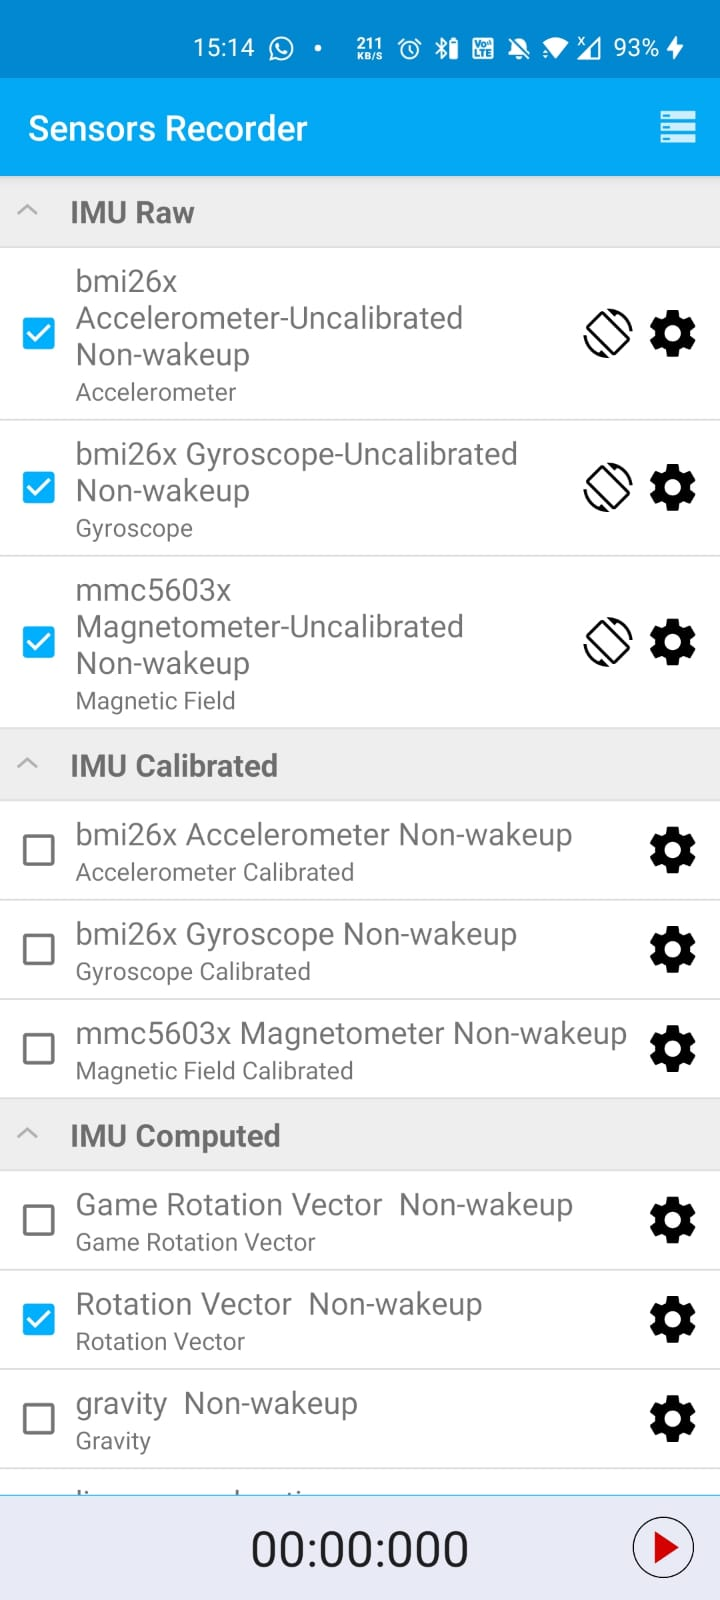
\includegraphics[width=0.6\linewidth]{images/recording_setting}
		\caption{Recording settings}
		\label{fig:recording_setting}
	\end{subfigure}
	\begin{subfigure}[t]{.45\textwidth}
		\centering
		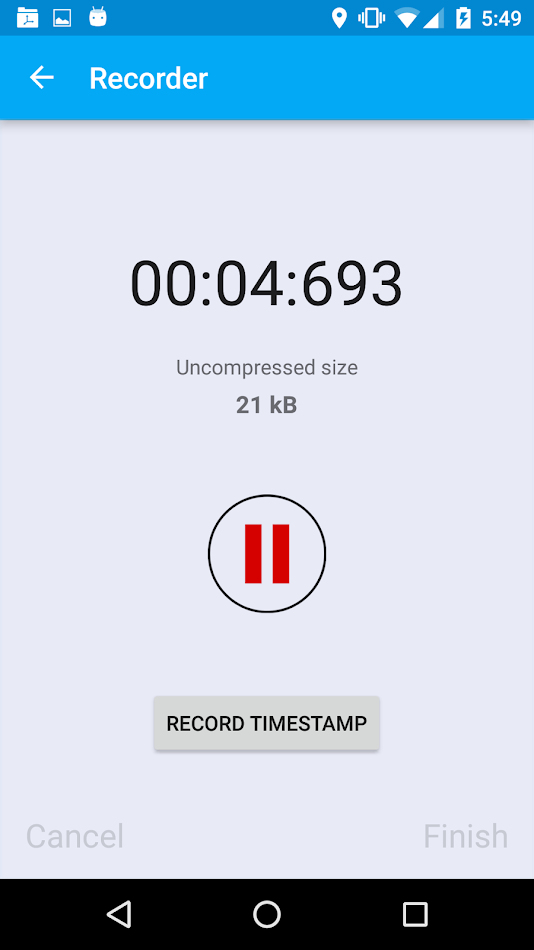
\includegraphics[width=0.7\linewidth]{images/recording_timestamp_button}
		\caption{Record timestamp button}
		\label{fig:recording_timestamp_button}
	\end{subfigure}
\caption{Indoor experiment android app configuration and button}
\end{figure}


\textbf{Postprocessing}

\begin{enumerate}
	\def\labelenumi{\arabic{enumi}.}
	\tightlist
	\item
	Calibrate walking around \ac{IMU} sensor data using calibration data
	\item
	Run calibrated walking around data through orientation estimation
	algorithm
	\item
	Compare result with orientation estimation made by the system and
	maybe even with the iphone 
	\item
	Determine steps and subsequent step length 
	\item
	Combine orientation information and step information to generate an
	estimated trajectory
	\item
	Use this estimated trajectory as input for the Particle Filter
	\item
	Using the video recording made during testing, manually indicate per
	step where on the blueprint you are. This will be used to determine
	the performance of the estimate of the \ac{SHS}system. 
\end{enumerate}


\chapter{SHS Trajectories}




\begin{figure}[H]
	\centering
	\begin{subfigure}[t]{.45\textwidth}
		\centering
		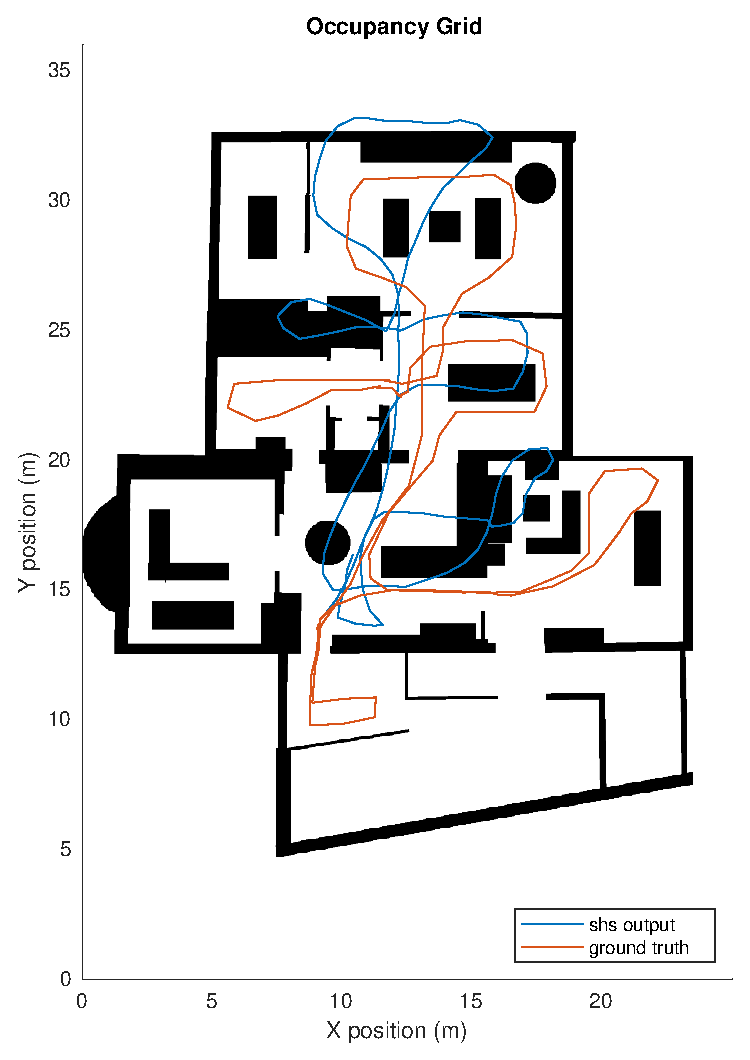
\includegraphics[width=0.9\linewidth]{images/20201029_1042_trial2_shs_1}
		\caption{trajectory comparison}
		\label{fig:trial2_on_map}
	\end{subfigure}
	\begin{subfigure}[t]{.45\textwidth}
		\centering
		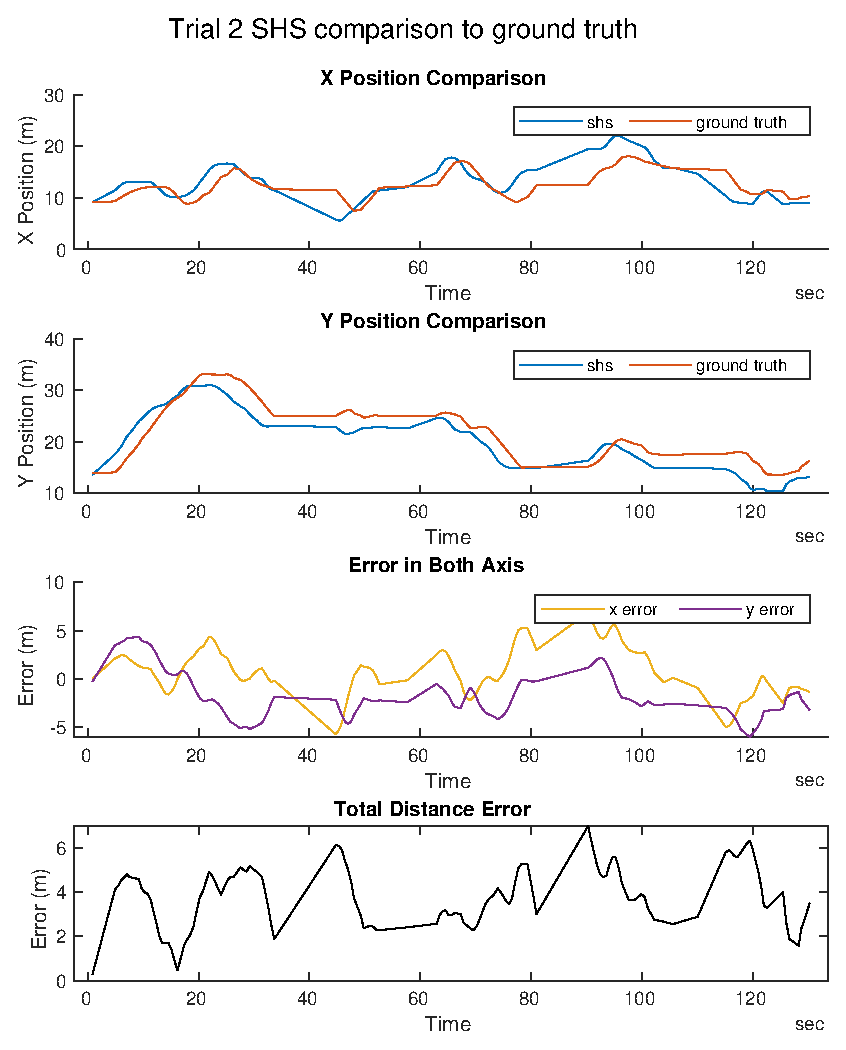
\includegraphics[width=\linewidth]{images/20201029_1042_trial2_shs_2}
		\caption{axis comparison}
		\label{fig:trial2_comparison}
	\end{subfigure}
	\setlength{\belowcaptionskip}{-20pt}
	\caption{Qualitative SHS comparison of trial 2 with ground truth}
	\label{fig:trial2_shs_gt_comparison}
\end{figure}


\chapter{Indoor Experiment Results}

\section{SHS-PF noise realization parameter search \textbf{without} door interactions}
\label{sec:app-shs_pf_noise_realization_no_detection}

\begin{figure}[H]
	\centering
	\includegraphics[width=0.7\linewidth]{"../../../Code and Datasets/SHS Code/pictures/20201202_1257_RMSE_between_video_trajectory_and_SHS-PF_for_Trial_NO_DETECTIONS1_1"}
	\setlength{\belowcaptionskip}{-20pt}
	\caption{}
	\label{fig:202012021257rmsebetweenvideotrajectoryandshs-pffortrialnodetections11}
\end{figure}
\begin{figure}[H]
	\centering
	\includegraphics[width=0.7\linewidth]{"../../../Code and Datasets/SHS Code/pictures/20201202_1257_RMSE_between_video_trajectory_and_SHS-PF_for_Trial_NO_DETECTIONS2_1"}
	\setlength{\belowcaptionskip}{-20pt}
	\caption{}
	\label{fig:202012021257rmsebetweenvideotrajectoryandshs-pffortrialnodetections21}
\end{figure}
\begin{figure}[H]
	\centering
	\includegraphics[width=0.7\linewidth]{"../../../Code and Datasets/SHS Code/pictures/20201202_1258_RMSE_between_video_trajectory_and_SHS-PF_for_Trial_NO_DETECTIONS3_1"}
	\setlength{\belowcaptionskip}{-20pt}
	\caption{}
	\label{fig:202012021258rmsebetweenvideotrajectoryandshs-pffortrialnodetections31}
\end{figure}
\begin{figure}[H]
	\centering
	\includegraphics[width=0.7\linewidth]{"../../../Code and Datasets/SHS Code/pictures/20201202_1259_RMSE_between_video_trajectory_and_SHS-PF_for_Trial_NO_DETECTIONS6_1"}
	\setlength{\belowcaptionskip}{-20pt}
	\caption{}
	\label{fig:202012021259rmsebetweenvideotrajectoryandshs-pffortrialnodetections61}
\end{figure}



\section{SHS-PF noise realization parameter search \textbf{with} door interactions}
\label{sec:app-shs_pf_noise_realization}


\begin{figure}[H]
	\centering
	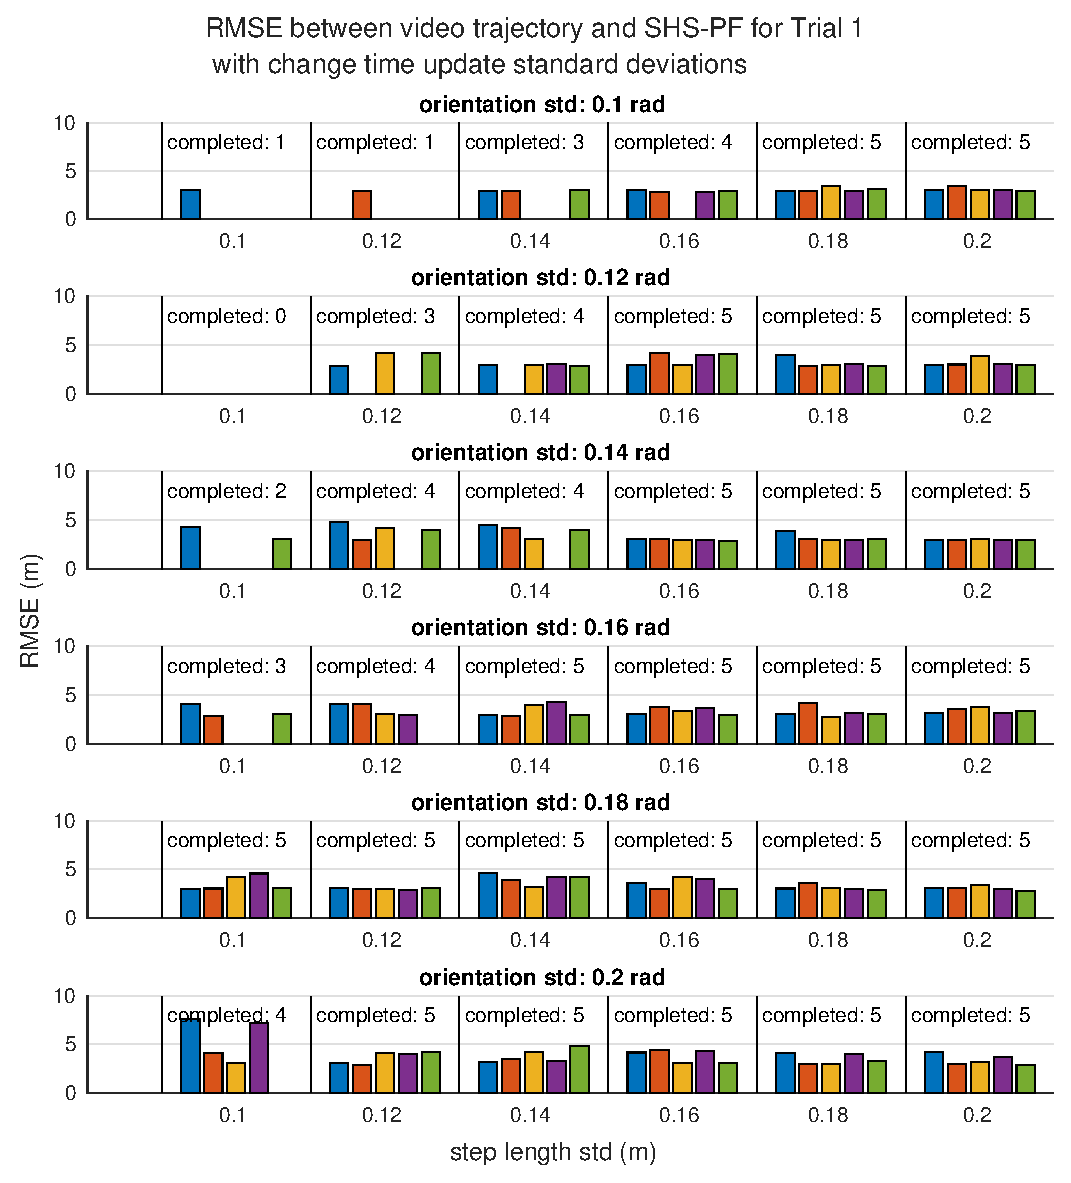
\includegraphics[width=0.6\linewidth]{images/20201201_0951_RMSE_between_video_trajectory_and_SHS-PF_for_Trial_1_1}
		\setlength{\belowcaptionskip}{-20pt}
	\caption{}
	\label{fig:202012010951rmsebetweenvideotrajectoryandshs-pffortrial11}
\end{figure}
\begin{figure}[H]
	\centering
	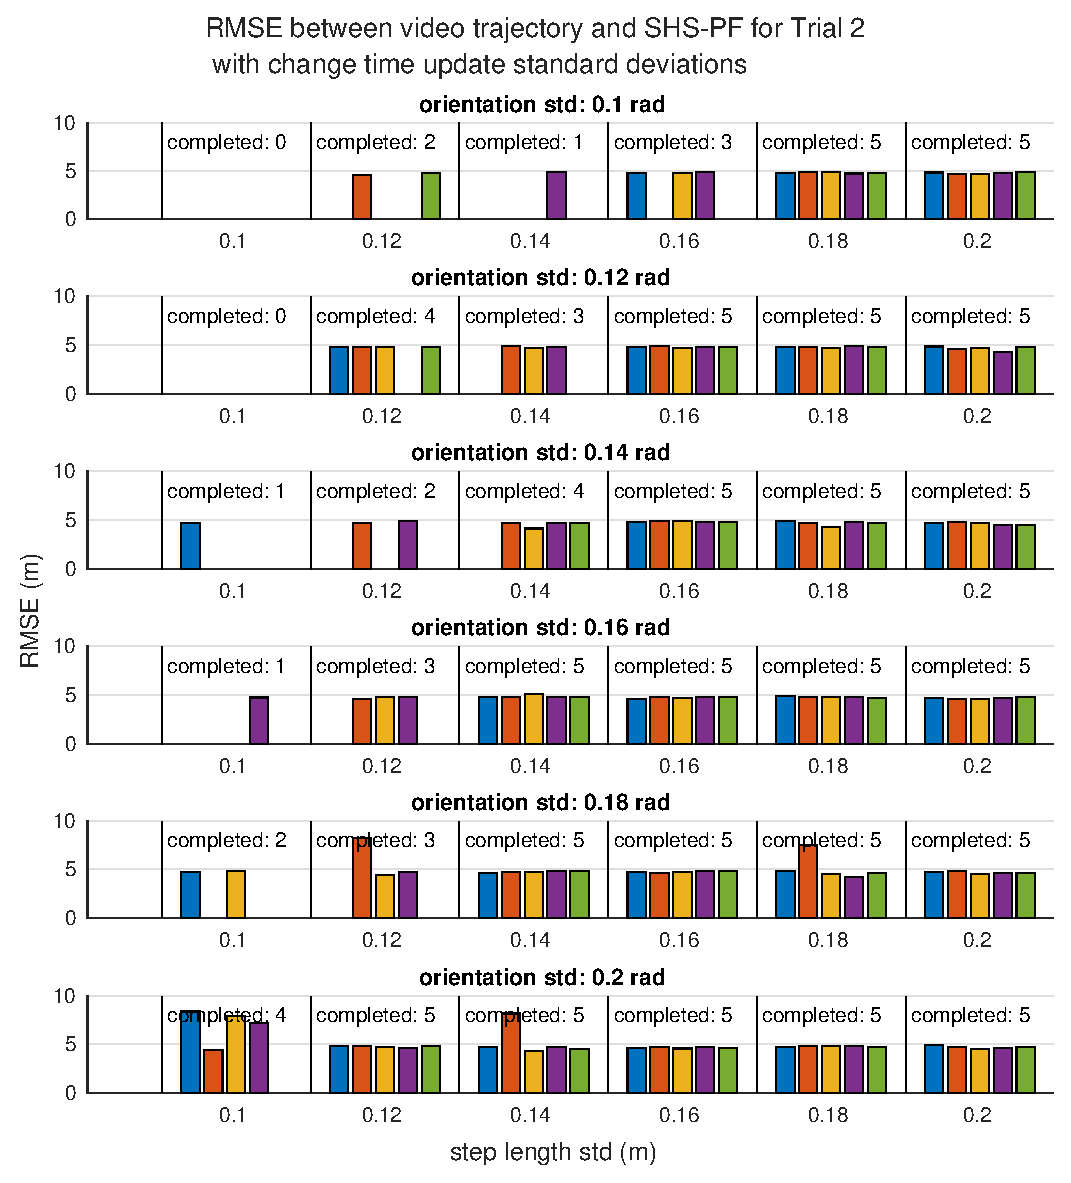
\includegraphics[width=0.6\linewidth]{images/20201201_0951_RMSE_between_video_trajectory_and_SHS-PF_for_Trial_2_1}
	\setlength{\belowcaptionskip}{-20pt}
	\caption{}
	\label{fig:202012010951rmsebetweenvideotrajectoryandshs-pffortrial21}
\end{figure}
\begin{figure}[H]
	\centering
	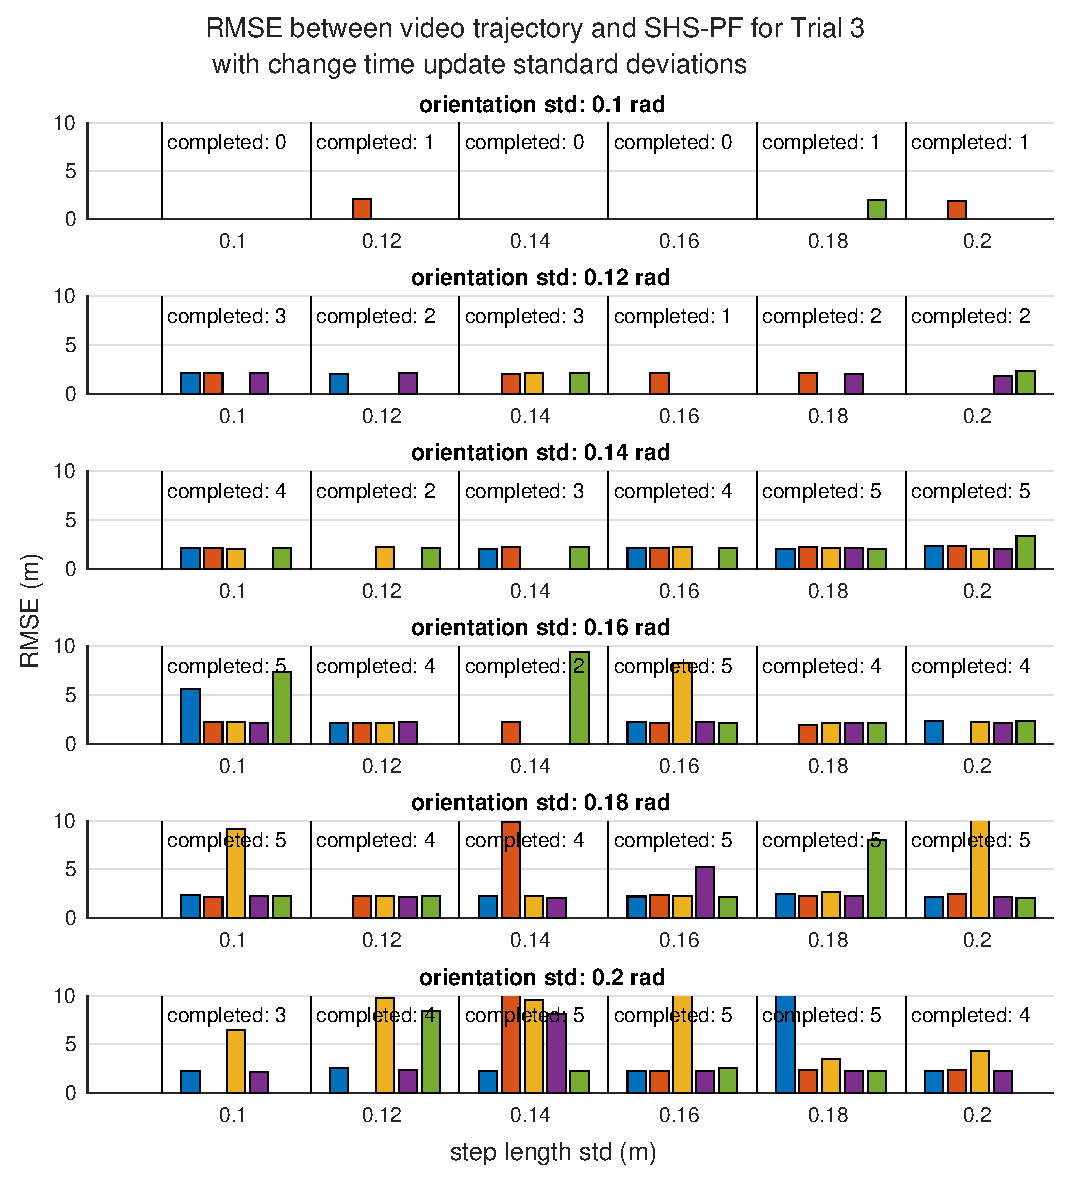
\includegraphics[width=0.6\linewidth]{images/20201201_0951_RMSE_between_video_trajectory_and_SHS-PF_for_Trial_3_1}
	\setlength{\belowcaptionskip}{-20pt}
	\caption{}
	\label{fig:202012010951rmsebetweenvideotrajectoryandshs-pffortrial31}
\end{figure}
\begin{figure}[H]
	\centering
	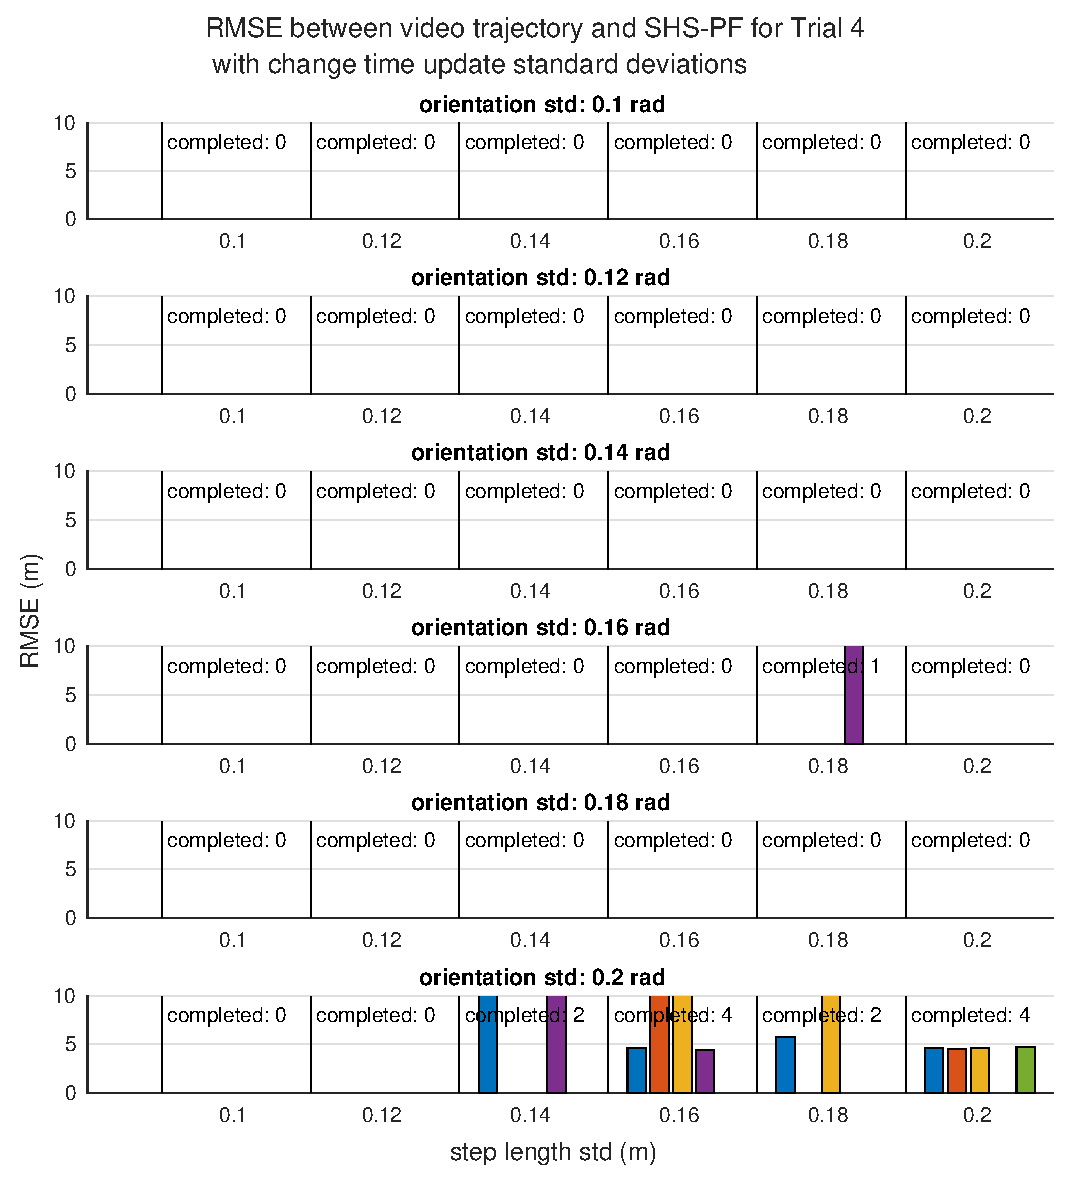
\includegraphics[width=0.6\linewidth]{images/20201201_0951_RMSE_between_video_trajectory_and_SHS-PF_for_Trial_4_1}
	\setlength{\belowcaptionskip}{-20pt}
	\caption{}
	\label{fig:202012010951rmsebetweenvideotrajectoryandshs-pffortrial41}
\end{figure}
\begin{figure}[H]
	\centering
	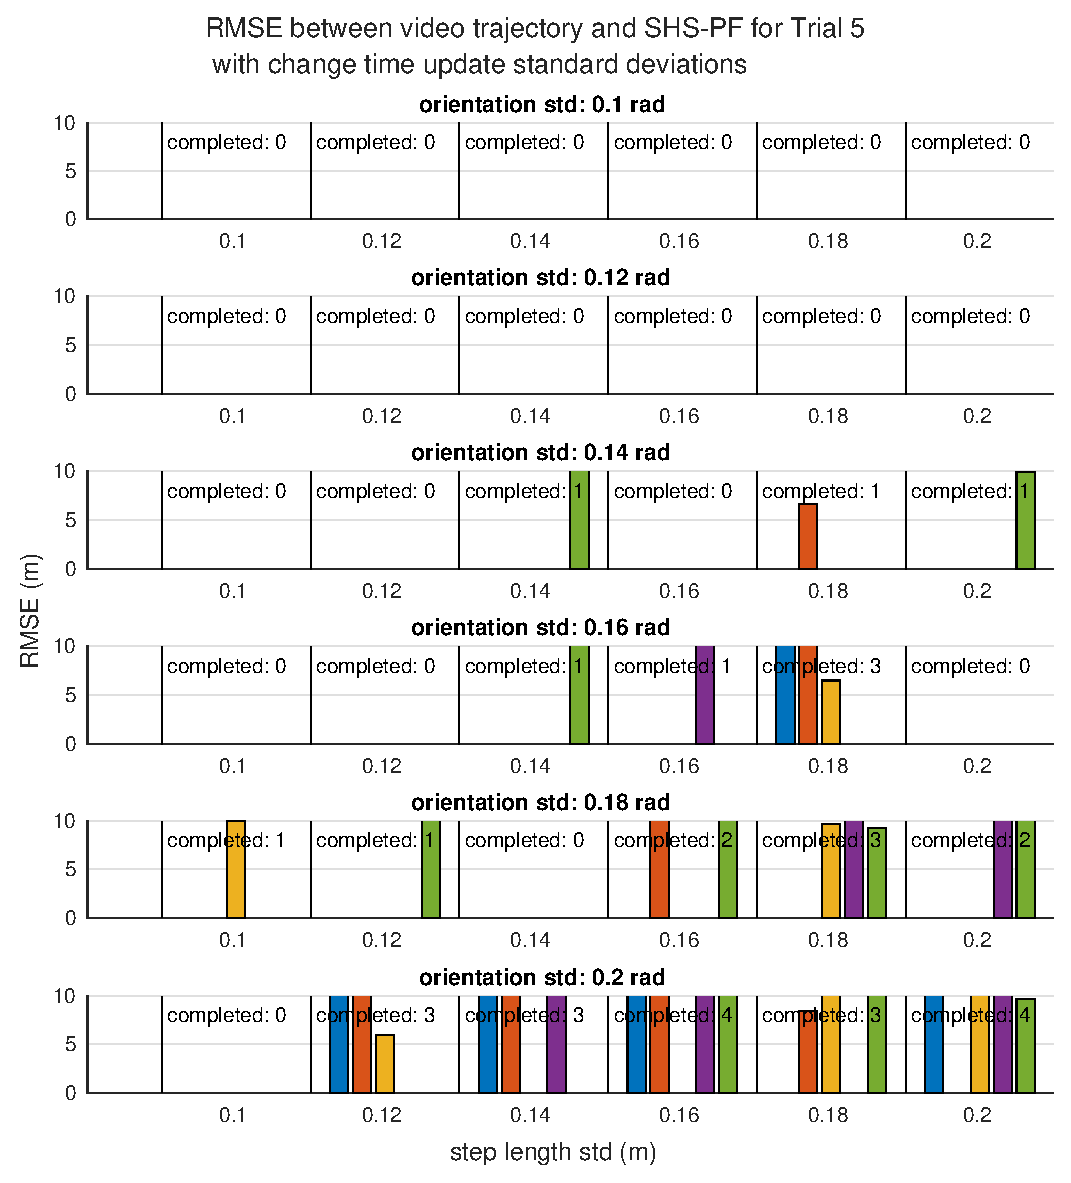
\includegraphics[width=0.6\linewidth]{images/20201201_0951_RMSE_between_video_trajectory_and_SHS-PF_for_Trial_5_1}
	\setlength{\belowcaptionskip}{-20pt}
	\caption{}
	\label{fig:202012010951rmsebetweenvideotrajectoryandshs-pffortrial51}
\end{figure}
\begin{figure}[H]
	\centering
	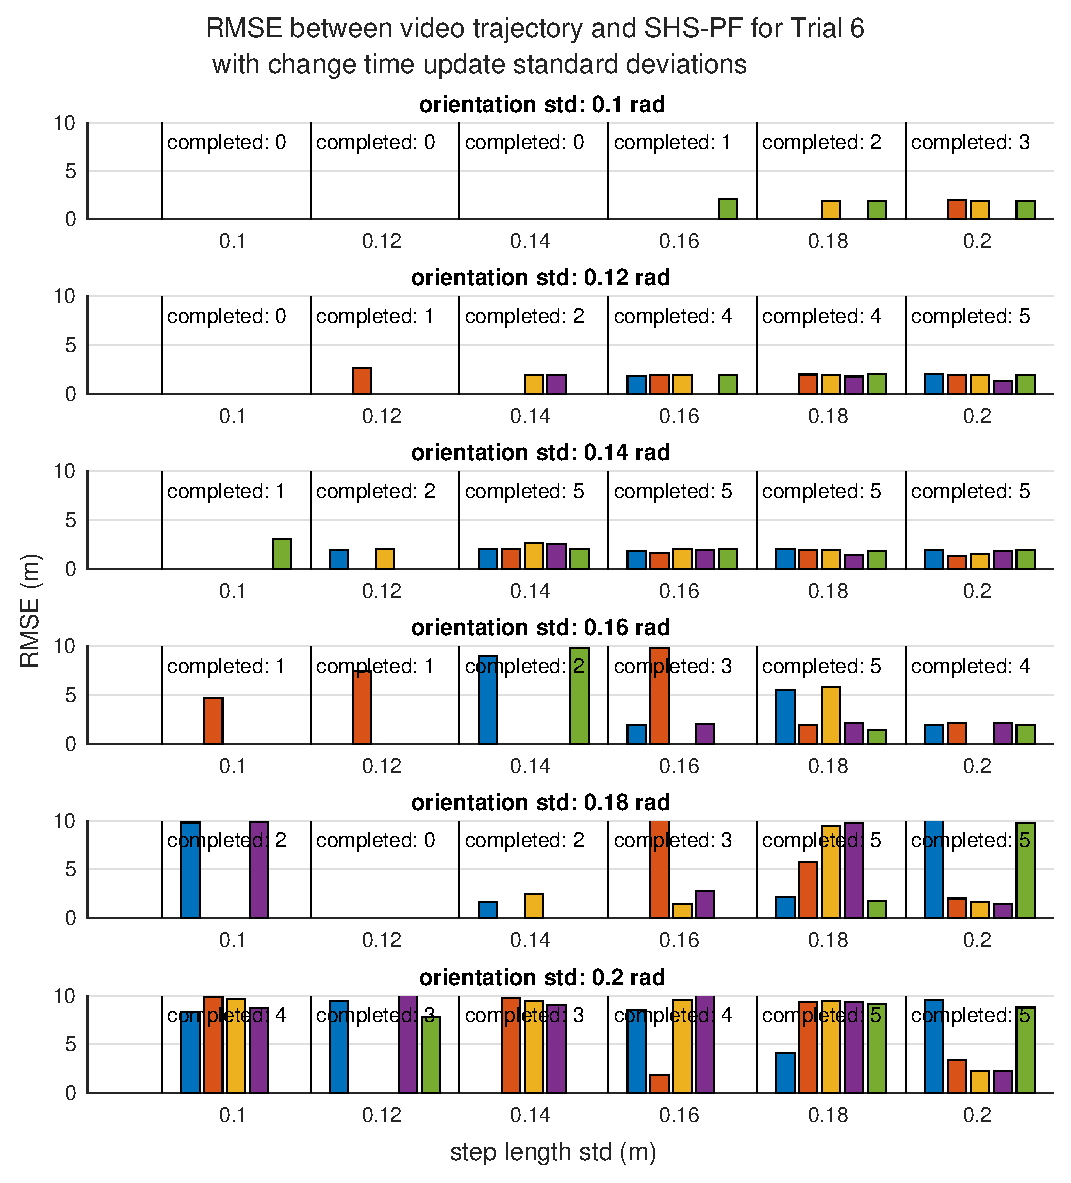
\includegraphics[width=0.6\linewidth]{images/20201201_0952_RMSE_between_video_trajectory_and_SHS-PF_for_Trial_6_1}
	\setlength{\belowcaptionskip}{-20pt}
	\caption{}
	\label{fig:202012010952rmsebetweenvideotrajectoryandshs-pffortrial61}
\end{figure}




\newpage
\section{SHS-PF Increasing Particle Number}
\label{app:SHS-PF trials}

\begin{figure}[H]
	\centering
	\begin{subfigure}[t]{.4\textwidth}
		\centering
		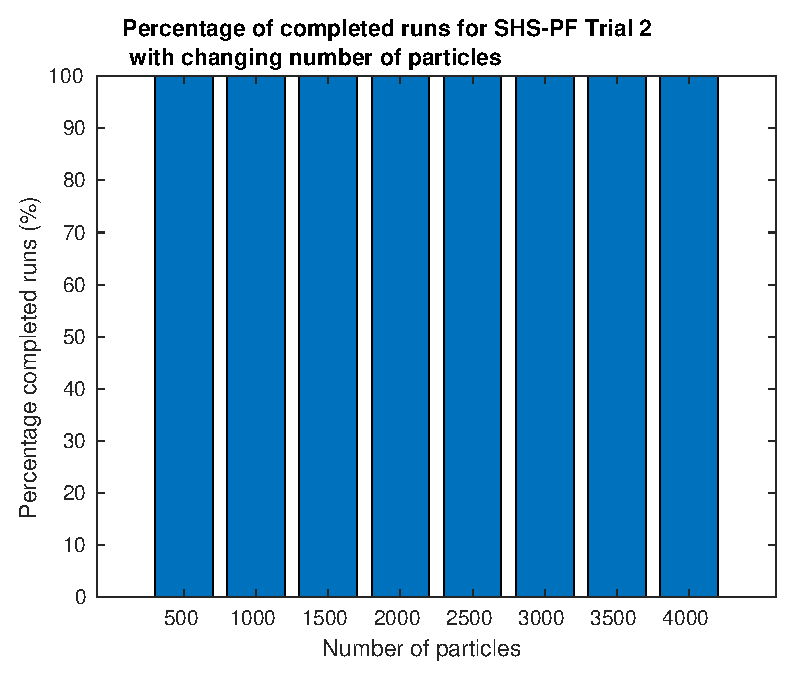
\includegraphics[width=\linewidth]{images/20201129_1147_Trial_2_nr_particles_1}
		\caption{Number of completed runs for SHS-PF with increasing number of particles.}
		\label{fig:trial2_nr_particles_completed}
	\end{subfigure} \quad
	\begin{subfigure}[t]{.4\textwidth}
		\centering
		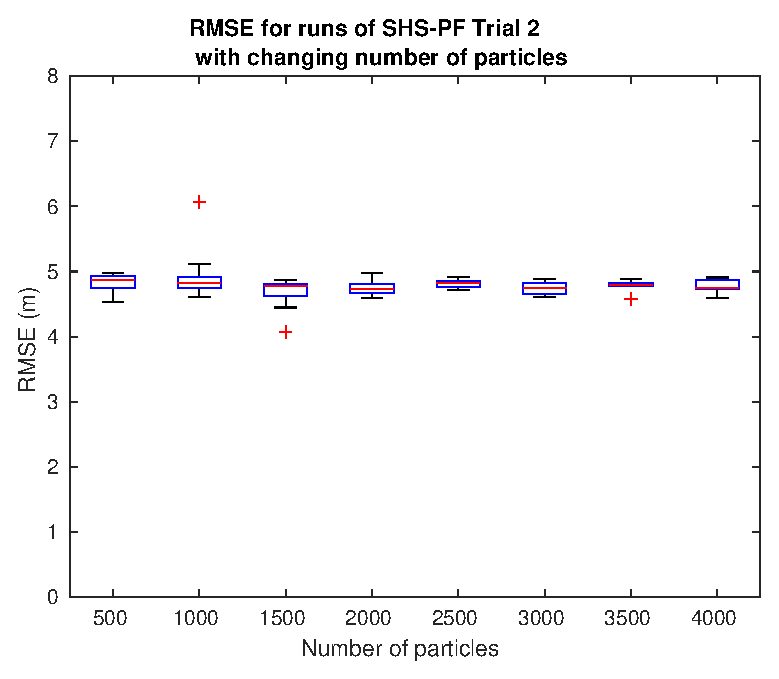
\includegraphics[width=\linewidth]{images/20201129_1154_Trial_2_RMSE_nr_particles_1}
		\caption{RMSE between video trajectory and SHS-PF with manually indicated door interaction, with increasing number of particles}
		\label{fig:trial2_nr_particles_RMSE}
	\end{subfigure}
	\label{fig:trial2_nr_particles}
	\caption{Increasing number of particles for SHS-PF in trial 2.}
\end{figure}

\begin{figure}[H]
	\centering
	\begin{subfigure}[t]{.4\textwidth}
		\centering
		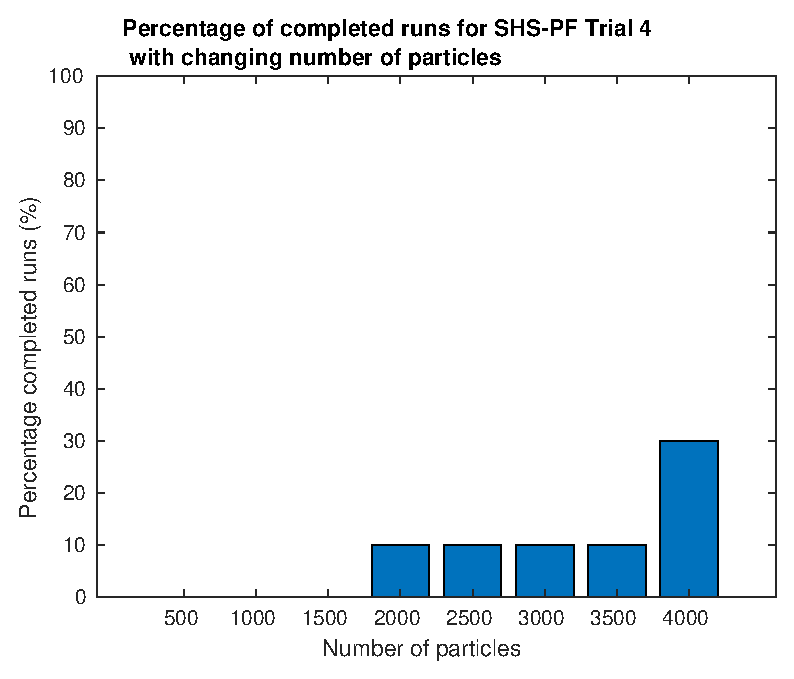
\includegraphics[width=\linewidth]{images/20201201_1625_Trial_4_nr_particles_1}
		\caption{Number of completed runs for SHS-PF with increasing number of particles.}
		\label{fig:trial4_nr_particles_completed}
	\end{subfigure} \quad
	\begin{subfigure}[t]{.4\textwidth}
		\centering
		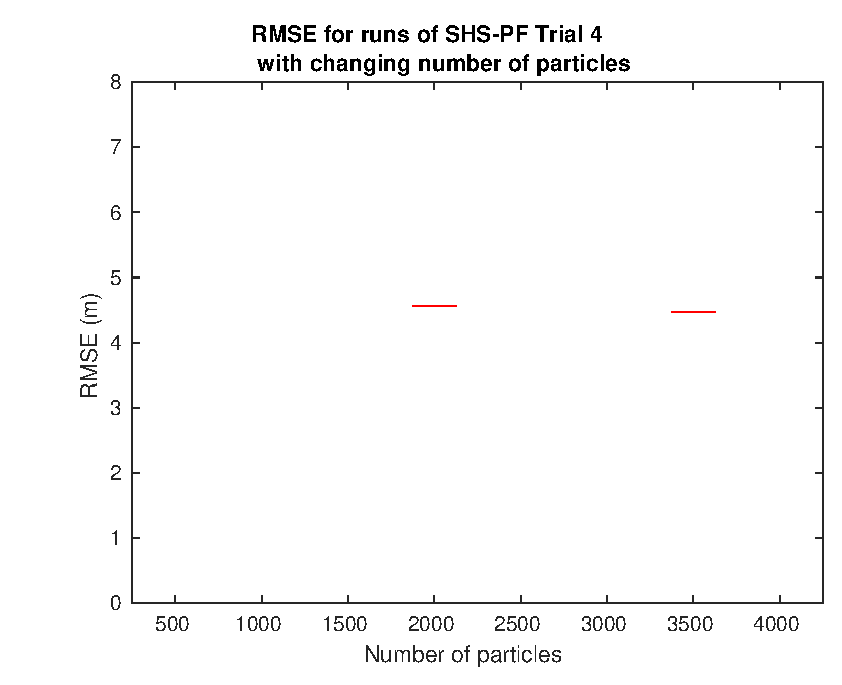
\includegraphics[width=\linewidth]{images/20201201_1622_Trial_4_RMSE_nr_particles_1}
		\caption{RMSE between video trajectory and SHS-PF with manually indicated door interaction, with increasing number of particles}
		\label{fig:trial4_nr_particles_RMSE}
	\end{subfigure}
	\label{fig:trial4_nr_particles}
	\caption{Increasing number of particles for SHS-PF in trial 4.}
\end{figure}

\begin{figure}[H]
	\centering
	\begin{subfigure}[t]{.4\textwidth}
		\centering
		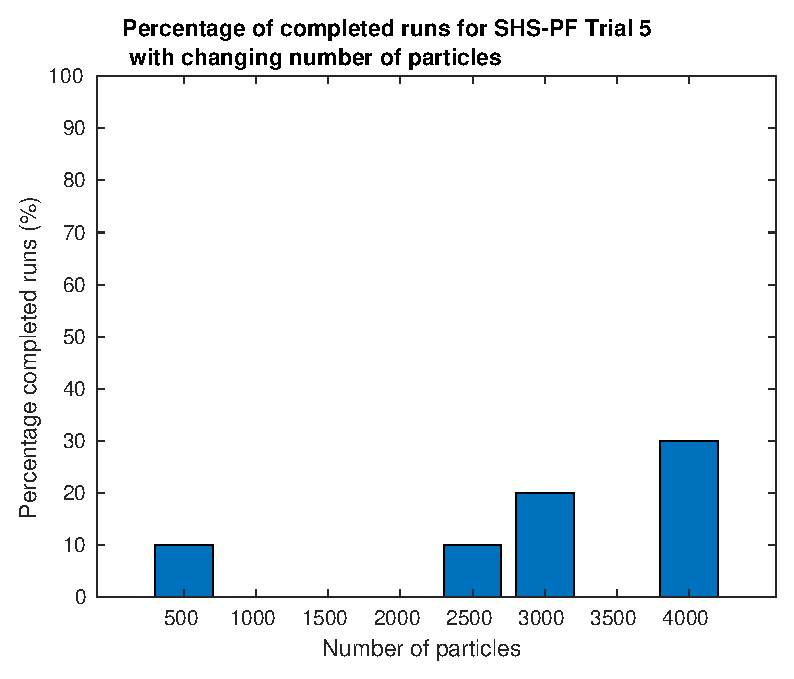
\includegraphics[width=\linewidth]{images/20201201_1625_Trial_5_nr_particles_1}
		\caption{Number of completed runs for SHS-PF with increasing number of particles.}
		\label{fig:trial5_nr_particles_completed}
	\end{subfigure} \quad
	\begin{subfigure}[t]{.4\textwidth}
		\centering
		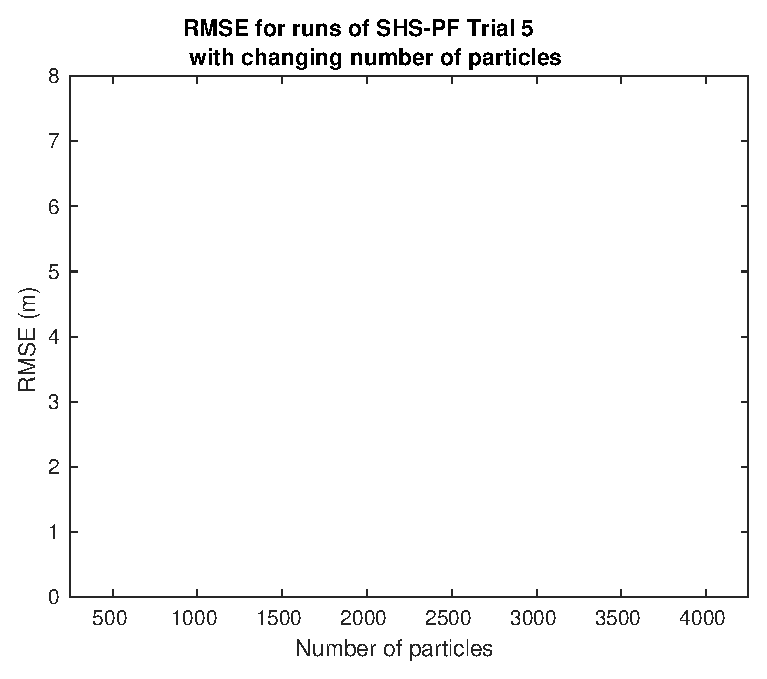
\includegraphics[width=\linewidth]{images/20201201_1622_Trial_5_RMSE_nr_particles_1}
		\caption{RMSE between video trajectory and SHS-PF with manually indicated door interaction, with increasing number of particles}
		\label{fig:trial5_nr_particles_RMSE}
	\end{subfigure}
	\label{fig:trial5_nr_particles}
	\caption{Increasing number of particles for SHS-PF in trial 5.}
\end{figure}

\begin{figure}[H]
	\centering
	\begin{subfigure}[t]{.4\textwidth}
		\centering
		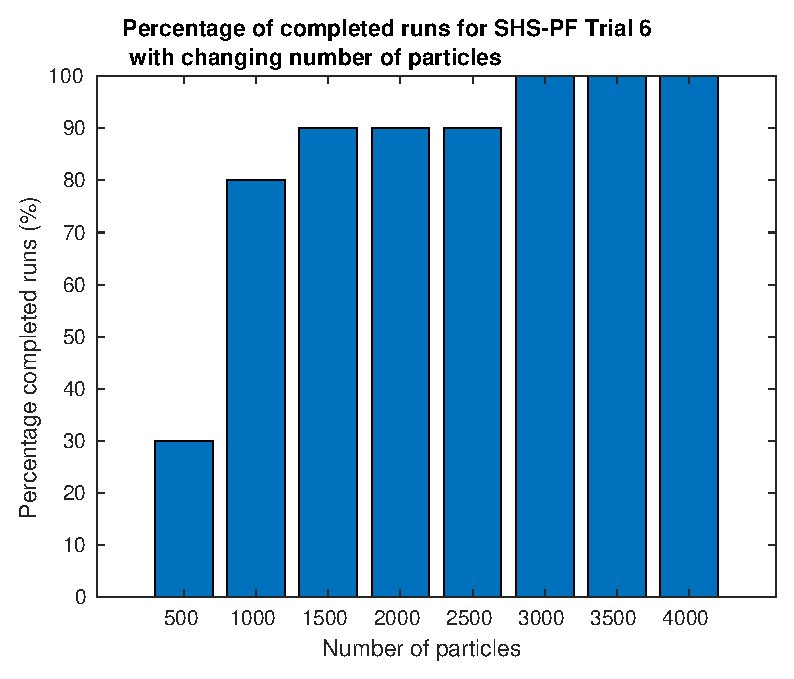
\includegraphics[width=\linewidth]{images/20201201_1625_Trial_6_nr_particles_1}
		\caption{Number of completed runs for SHS-PF with increasing number of particles.}
		\label{fig:trial6_nr_particles_completed}
	\end{subfigure} \quad
	\begin{subfigure}[t]{.4\textwidth}
		\centering
		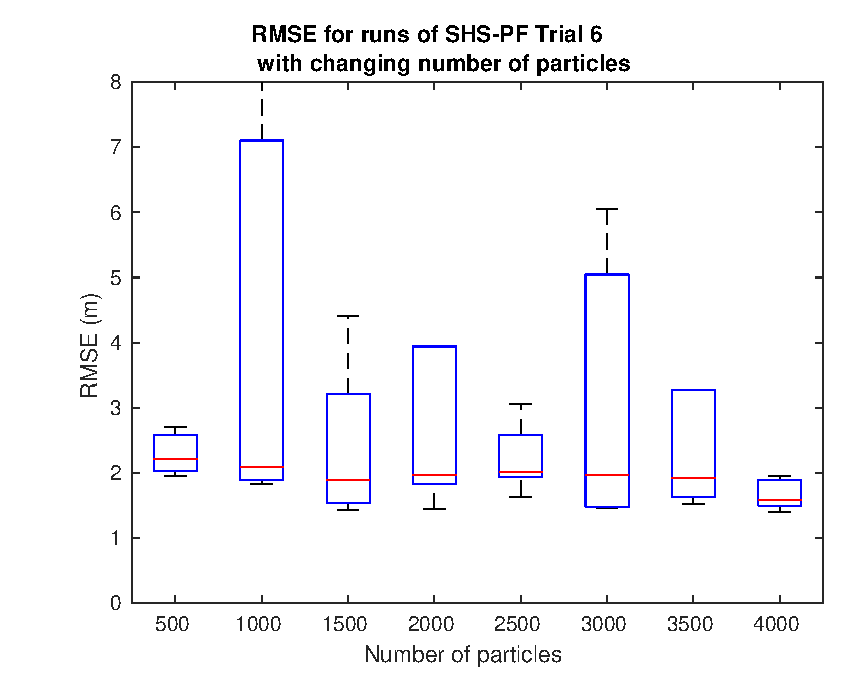
\includegraphics[width=\linewidth]{images/20201201_1622_Trial_6_RMSE_nr_particles_1}
		\caption{RMSE between video trajectory and SHS-PF with manually indicated door interaction, with increasing number of particles}
		\label{fig:trial6_nr_particles_RMSE}
	\end{subfigure}
	\label{fig:trial6_nr_particles}
	\caption{Increasing number of particles for SHS-PF in trial 6.}
\end{figure}

\newgeometry{left=3cm,bottom=0.1cm}
\section{Door Interaction Detection using Smartphone Accelerometer Data}
\label{sec:app-door_interaction_detection}
\begin{figure}[H]
	\centering
	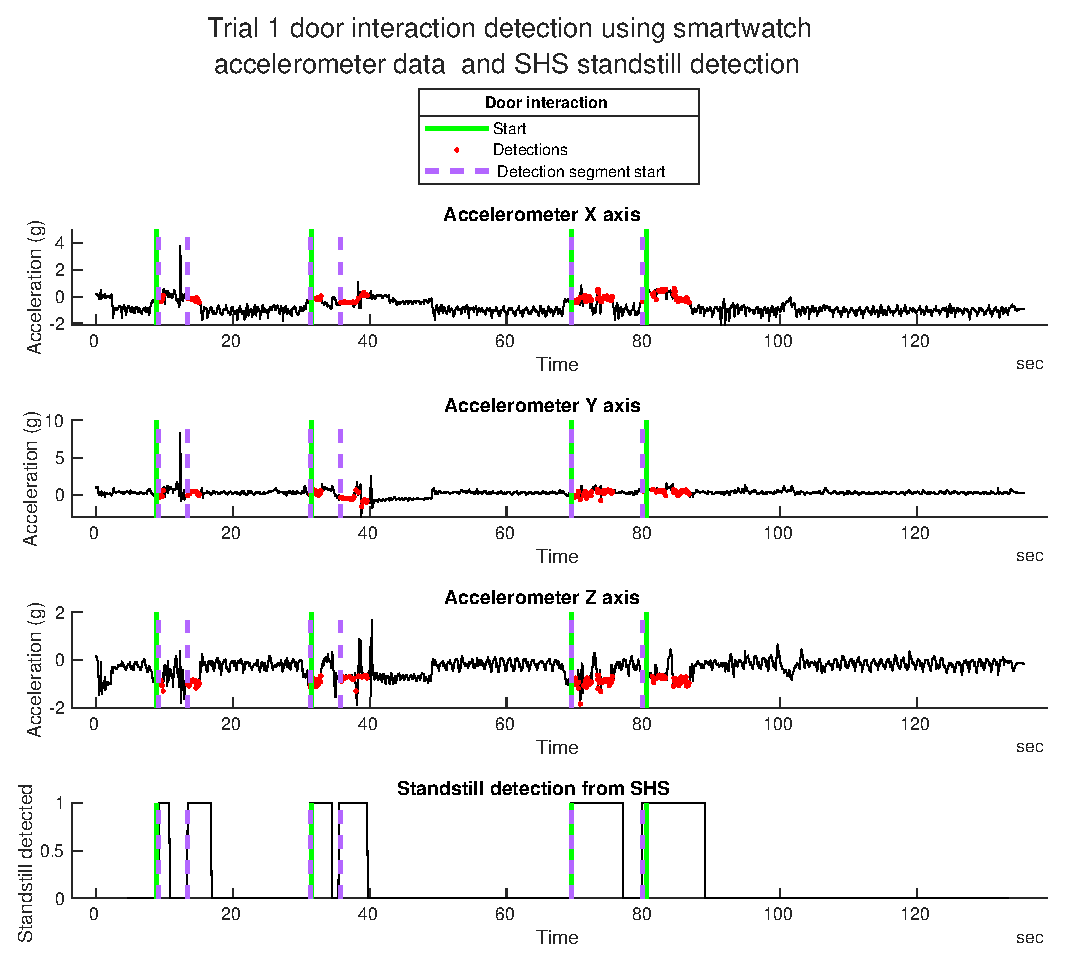
\includegraphics[width=0.8\linewidth]{images/20201201_1504_Trial_1_door_interaction_detection_using_smartwatch_1}
	\setlength{\belowcaptionskip}{-20pt}
	\caption{Trial 1 door interaction detection using smartwatch accelerometer data.}
	\label{fig:202011292139trial1doorinteractiondetectionusingsmartwatch1}
\end{figure}
\begin{figure}[H]
	\centering
	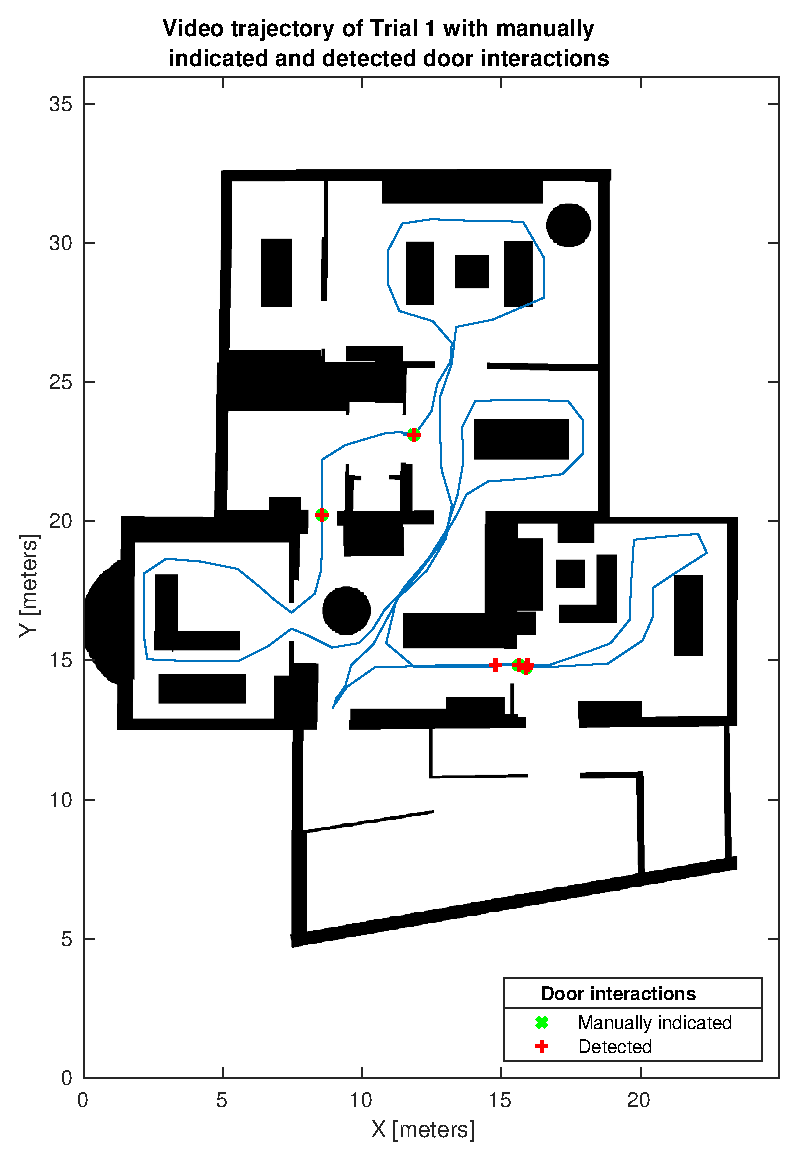
\includegraphics[width=0.7\linewidth]{images/20201129_2329_video_traj_Trial_1_door_detect_vs_manual_1}
	\setlength{\belowcaptionskip}{-20pt}
	\caption{Video trajectory for trial 1 with markers indicating position at time points when door interactions are either indicated manually or detected.}
	\label{fig:202011292329videotrajtrial1doordetectvsmanual1}
\end{figure}
\restoregeometry



\begin{figure}[H]
	\centering
	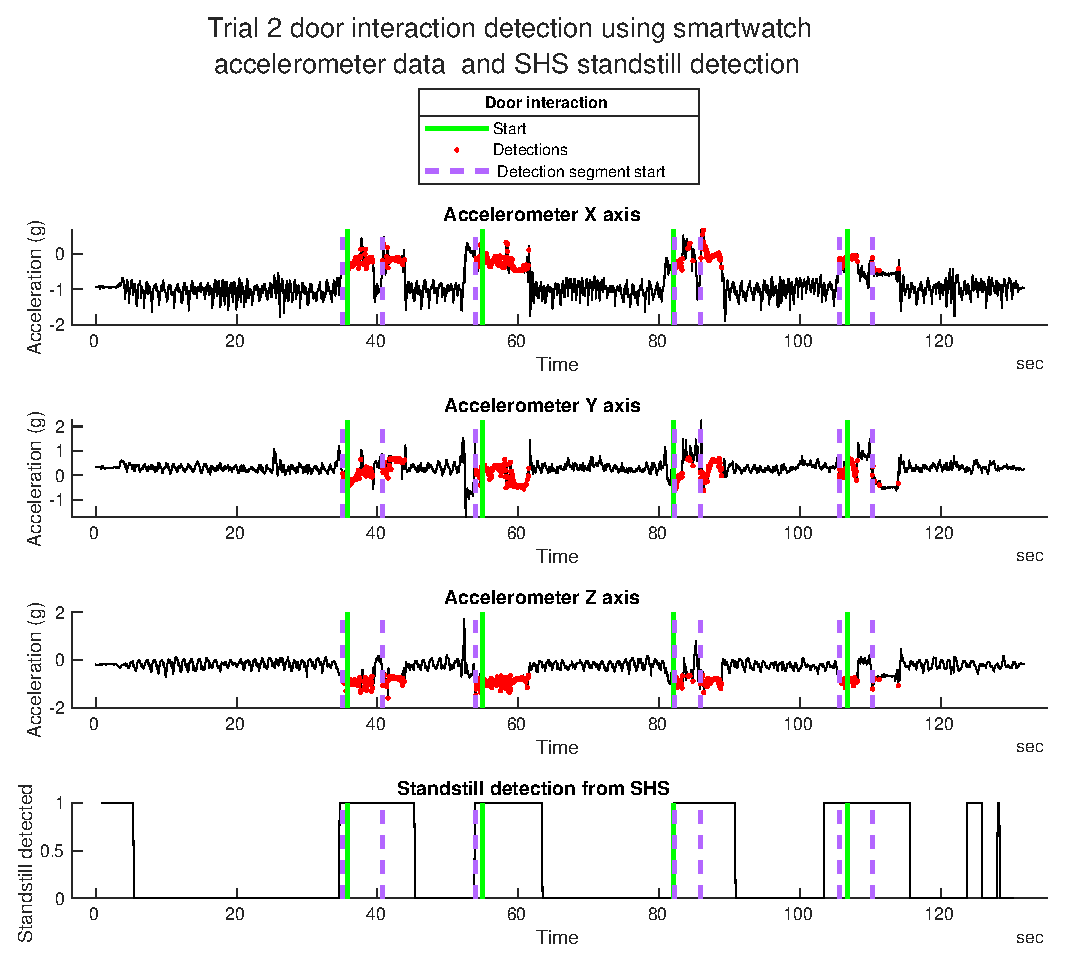
\includegraphics[width=0.8\linewidth]{images/20201201_1504_Trial_2_door_interaction_detection_using_smartwatch_1}
	\setlength{\belowcaptionskip}{-20pt}
	\caption{Trial 2 door interaction detection using smartwatch accelerometer data.}
	\label{fig:202011292139trial2doorinteractiondetectionusingsmartwatch1}
\end{figure}
\begin{figure}[H]
	\centering
	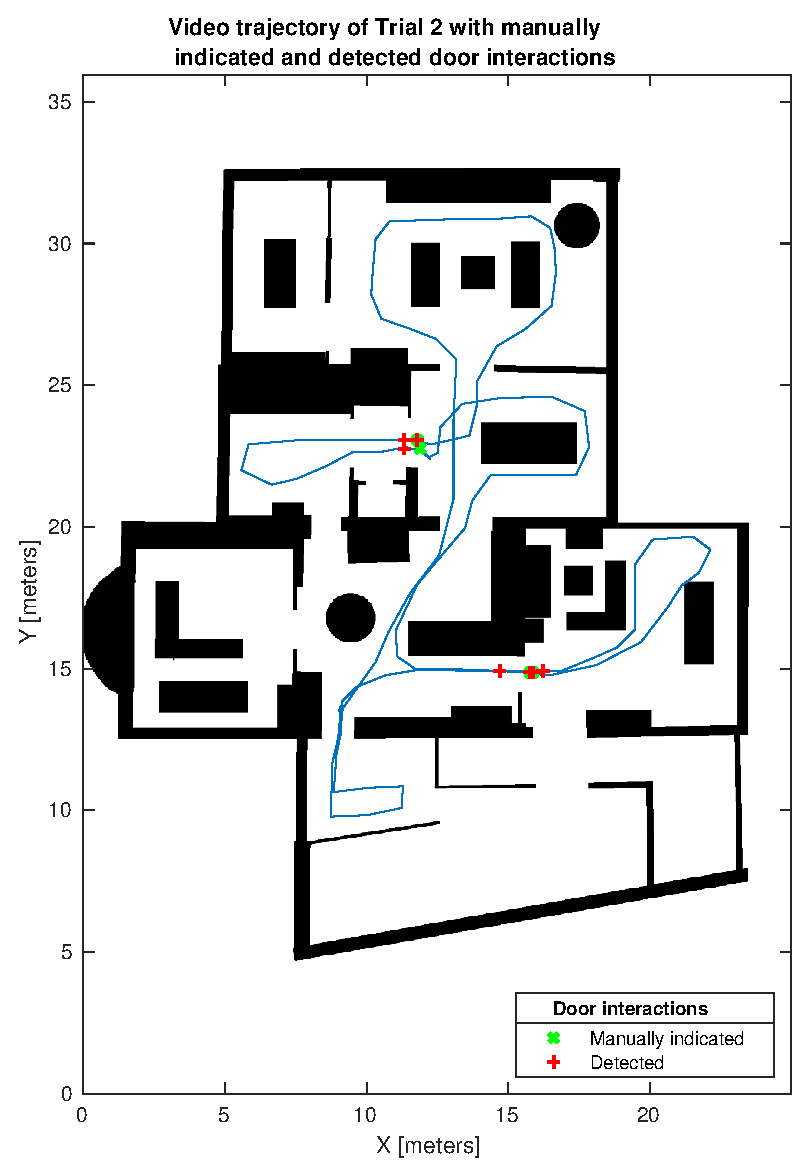
\includegraphics[width=0.7\linewidth]{images/20201129_2330_video_traj_Trial_2_door_detect_vs_manual_1}
	\setlength{\belowcaptionskip}{-20pt}
	\caption{Video trajectory for trial 2 with markers indicating position at time points when door interactions are either indicated manually or detected.}
	\label{fig:202011292330videotrajtrial2doordetectvsmanual1}
\end{figure}


\begin{figure}[H]
	\centering
	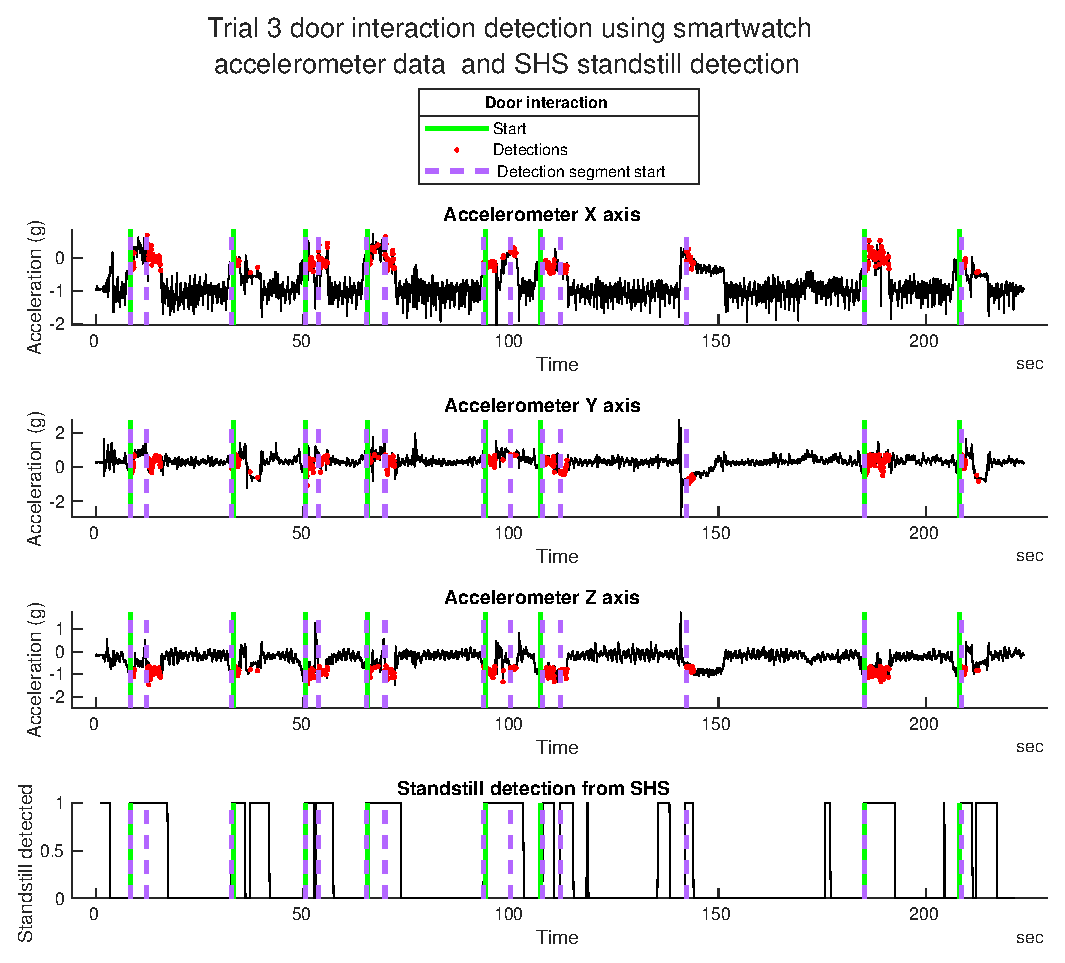
\includegraphics[width=0.8\linewidth]{images/20201201_1505_Trial_3_door_interaction_detection_using_smartwatch_1}
	\setlength{\belowcaptionskip}{-20pt}
	\caption{Trial 3 door interaction detection using smartwatch accelerometer data.}
	\label{fig:202011292139trial3doorinteractiondetectionusingsmartwatch1}
\end{figure}

\begin{figure}[H]
	\centering
	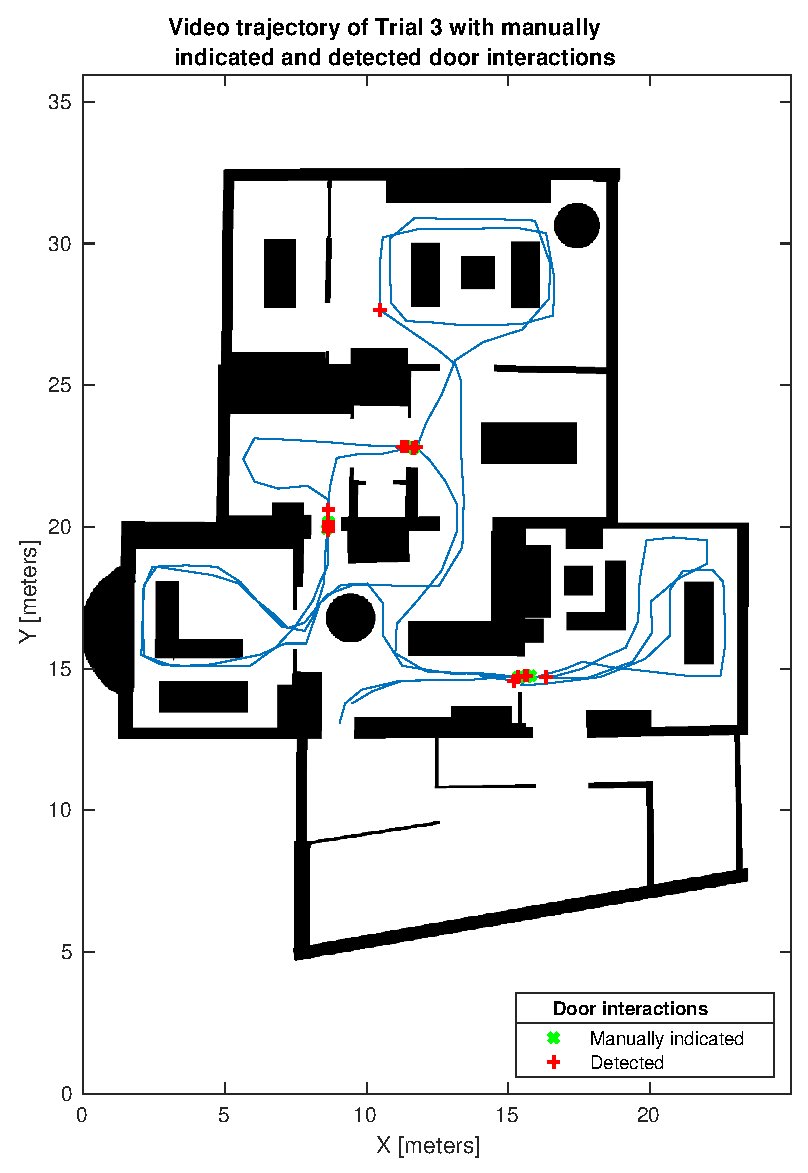
\includegraphics[width=0.7\linewidth]{images/20201129_2330_video_traj_Trial_3_door_detect_vs_manual_1}
	\setlength{\belowcaptionskip}{-20pt}
	\caption{Video trajectory for trial 3 with markers indicating position at time points when door interactions are either indicated manually or detected.}
	\label{fig:202011292330videotrajtrial3doordetectvsmanual1}
\end{figure}


\begin{figure}[H]
	\centering
	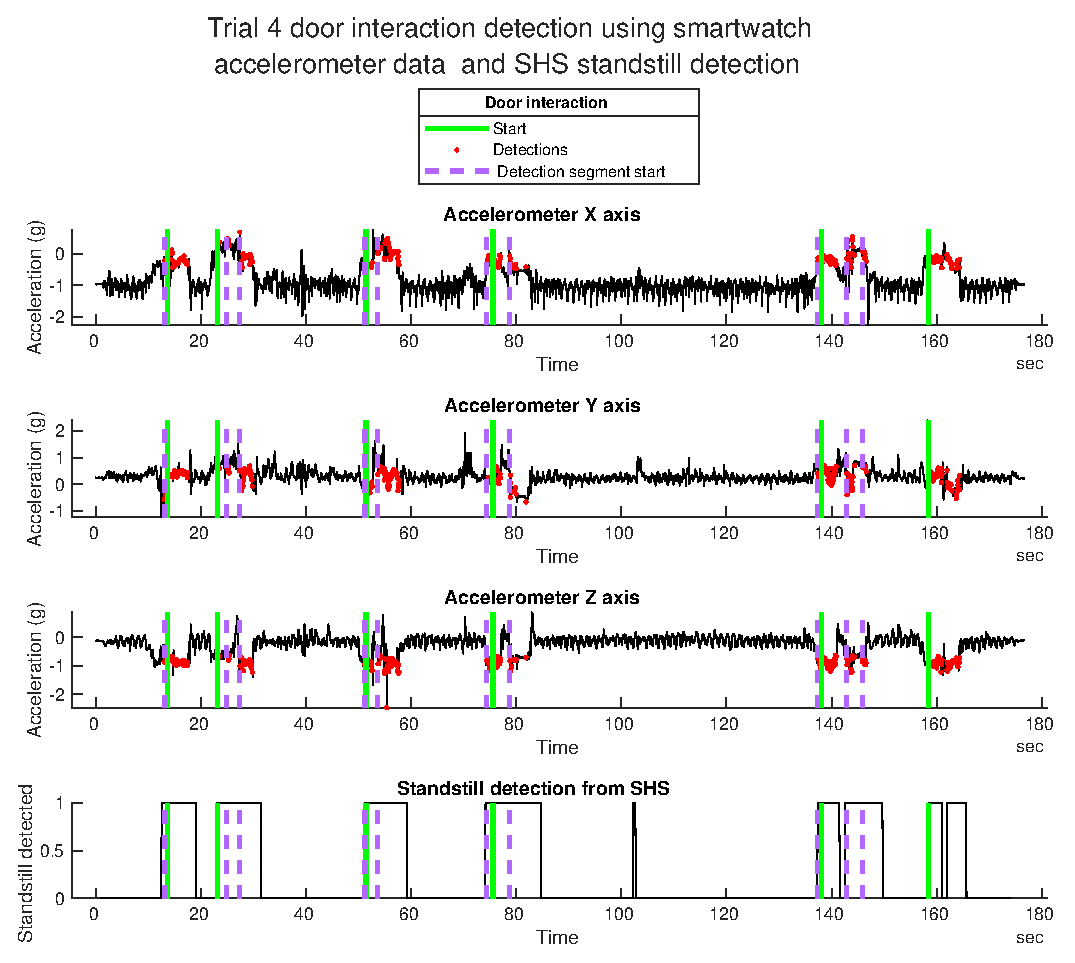
\includegraphics[width=0.8\linewidth]{images/20201201_1506_Trial_4_door_interaction_detection_using_smartwatch_1}
	\setlength{\belowcaptionskip}{-20pt}
	\caption{Trial 4 door interaction detection using smartwatch accelerometer data.}
	\label{fig:202011292140trial4doorinteractiondetectionusingsmartwatch1}
\end{figure}

\begin{figure}[H]
	\centering
	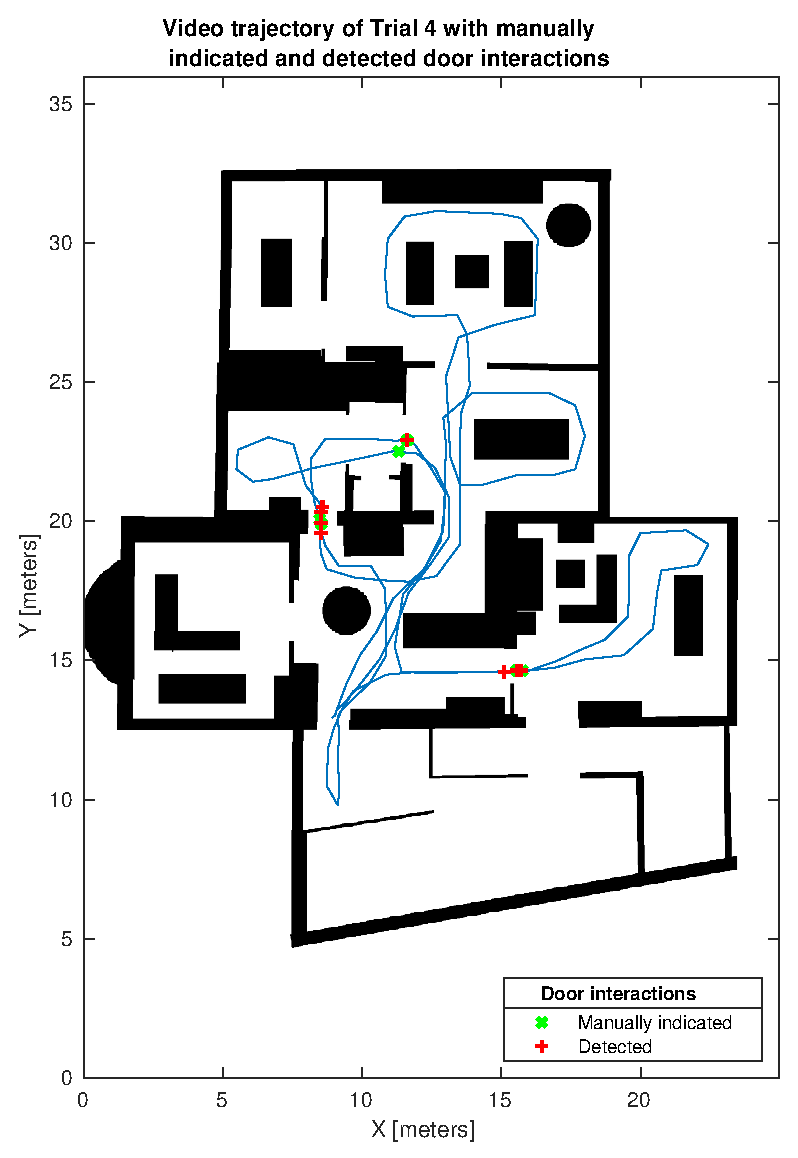
\includegraphics[width=0.7\linewidth]{images/20201129_2331_video_traj_Trial_4_door_detect_vs_manual_1}
	\setlength{\belowcaptionskip}{-20pt}
	\caption{Video trajectory for trial 4 with markers indicating position at time points when door interactions are either indicated manually or detected.}
	\label{fig:202011292331videotrajtrial4doordetectvsmanual1}
\end{figure}


\begin{figure}[H]
	\centering
	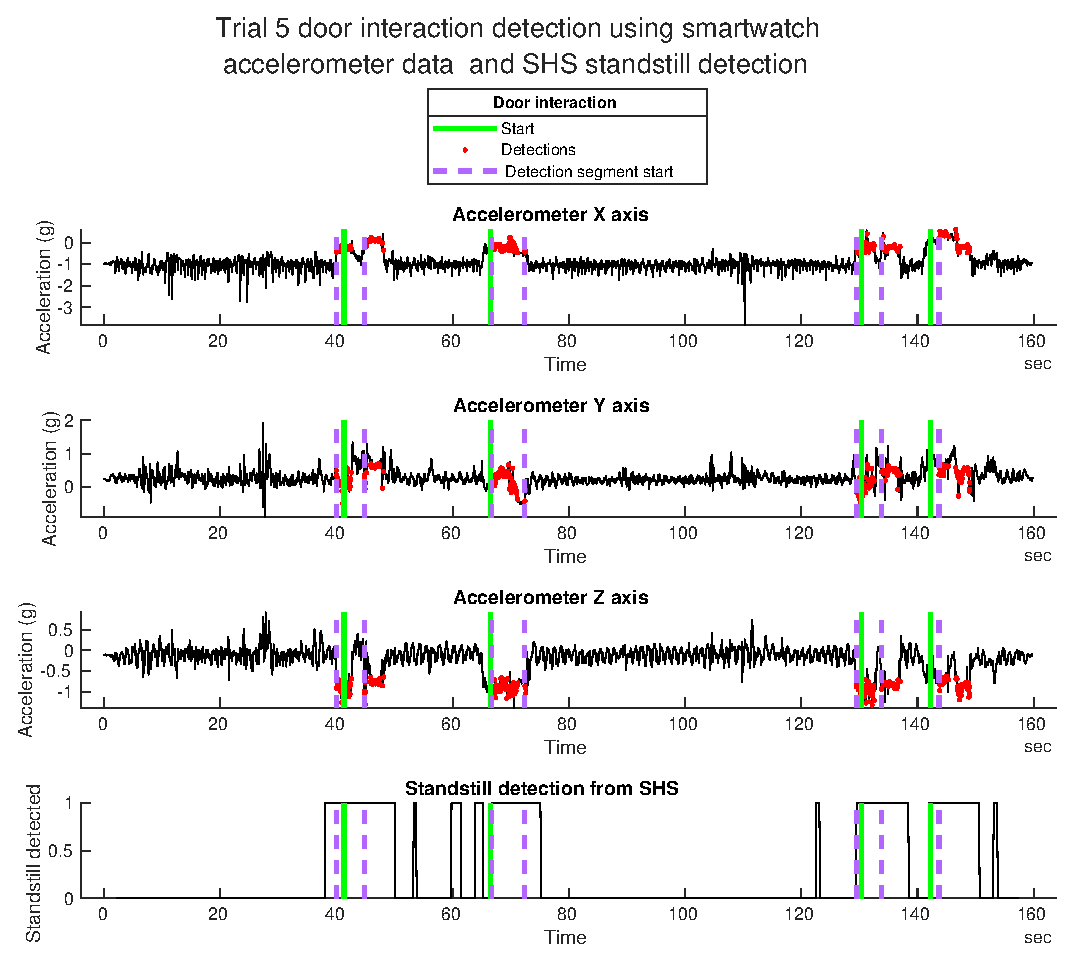
\includegraphics[width=0.8\linewidth]{images/20201201_1506_Trial_5_door_interaction_detection_using_smartwatch_1}
	\setlength{\belowcaptionskip}{-20pt}
	\caption{Trial 5 door interaction detection using smartwatch accelerometer data.}
	\label{fig:202011292141trial5doorinteractiondetectionusingsmartwatch1}
\end{figure}
\begin{figure}[H]
	\centering
	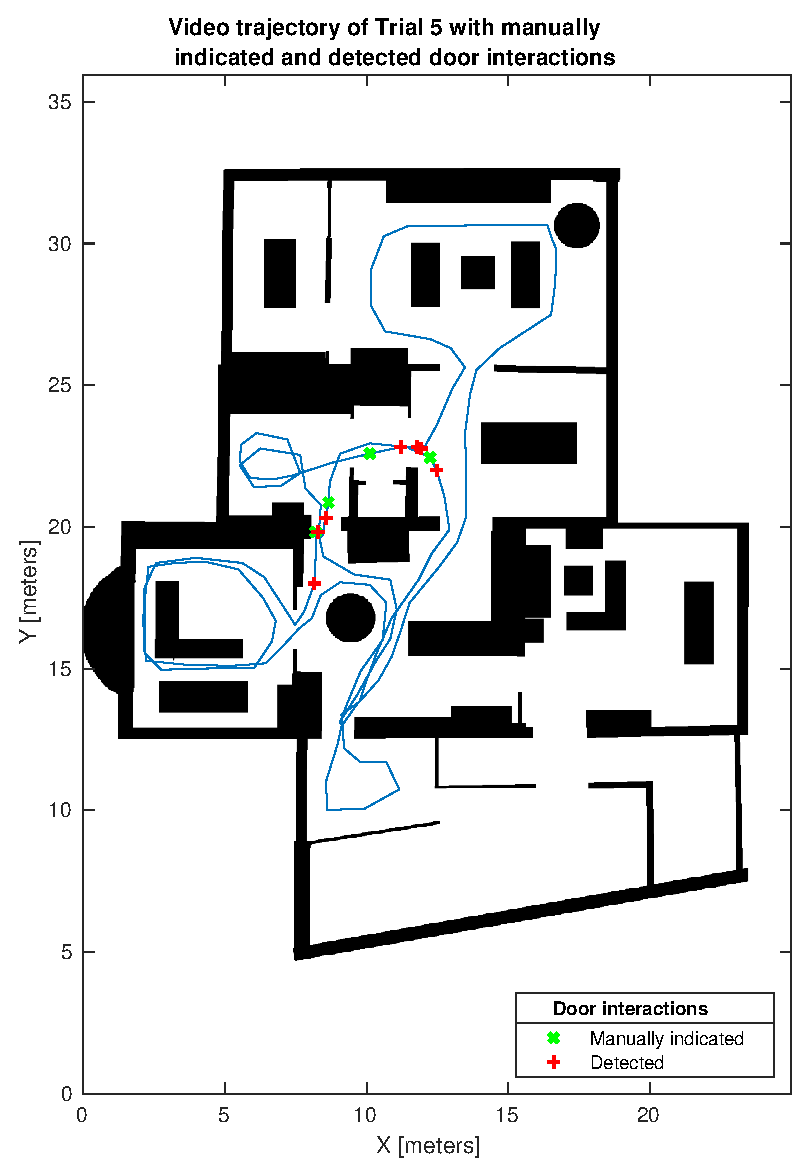
\includegraphics[width=0.7\linewidth]{images/20201129_2331_video_traj_Trial_5_door_detect_vs_manual_1}
	\setlength{\belowcaptionskip}{-20pt}
	\caption{Video trajectory for trial 5 with markers indicating position at time points when door interactions are either indicated manually or detected.}
	\label{fig:202011292331videotrajtrial5doordetectvsmanual1}
\end{figure}



\begin{figure}[H]
	\centering
	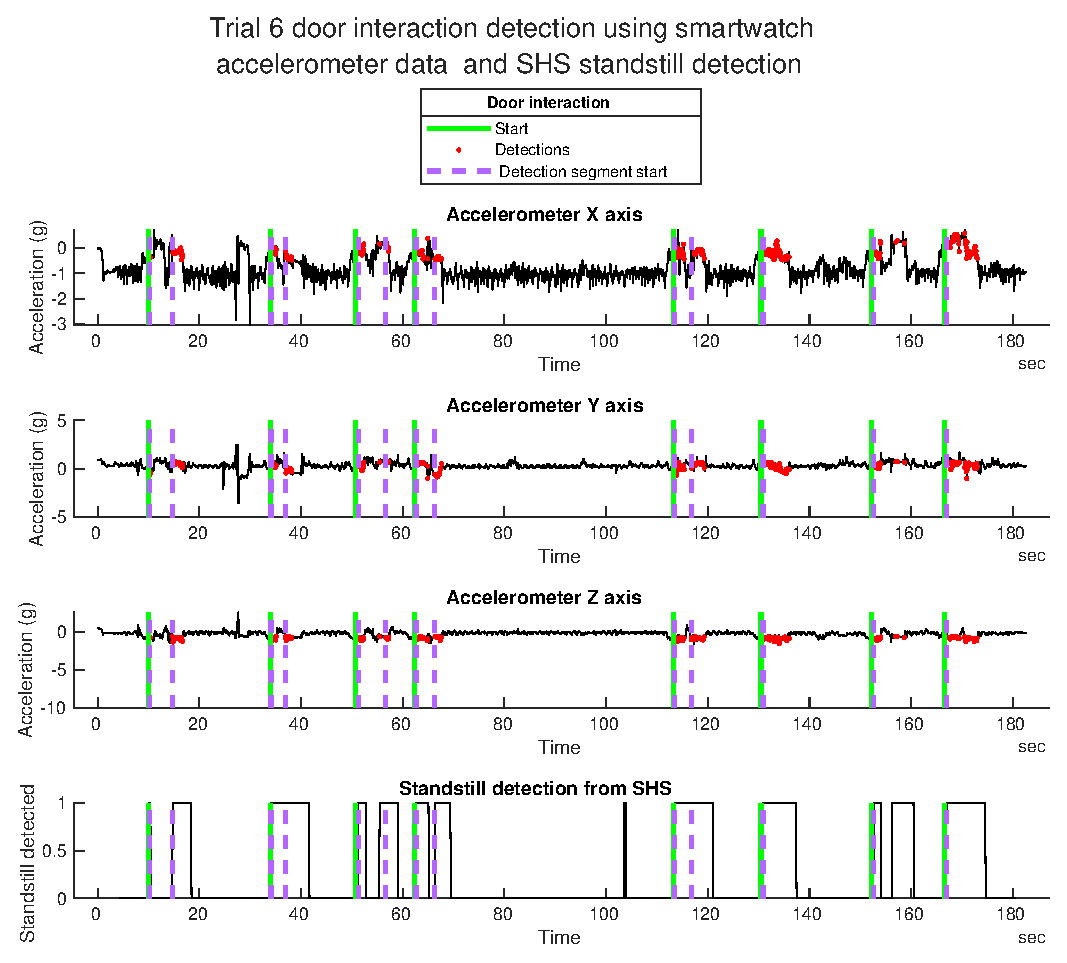
\includegraphics[width=0.8\linewidth]{images/20201201_1506_Trial_6_door_interaction_detection_using_smartwatch_1}
	\setlength{\belowcaptionskip}{-20pt}
	\caption{Trial 6 door interaction detection using smartwatch accelerometer data.}
	\label{fig:202011292141trial6doorinteractiondetectionusingsmartwatch1}
\end{figure}
\begin{figure}[H]
	\centering
	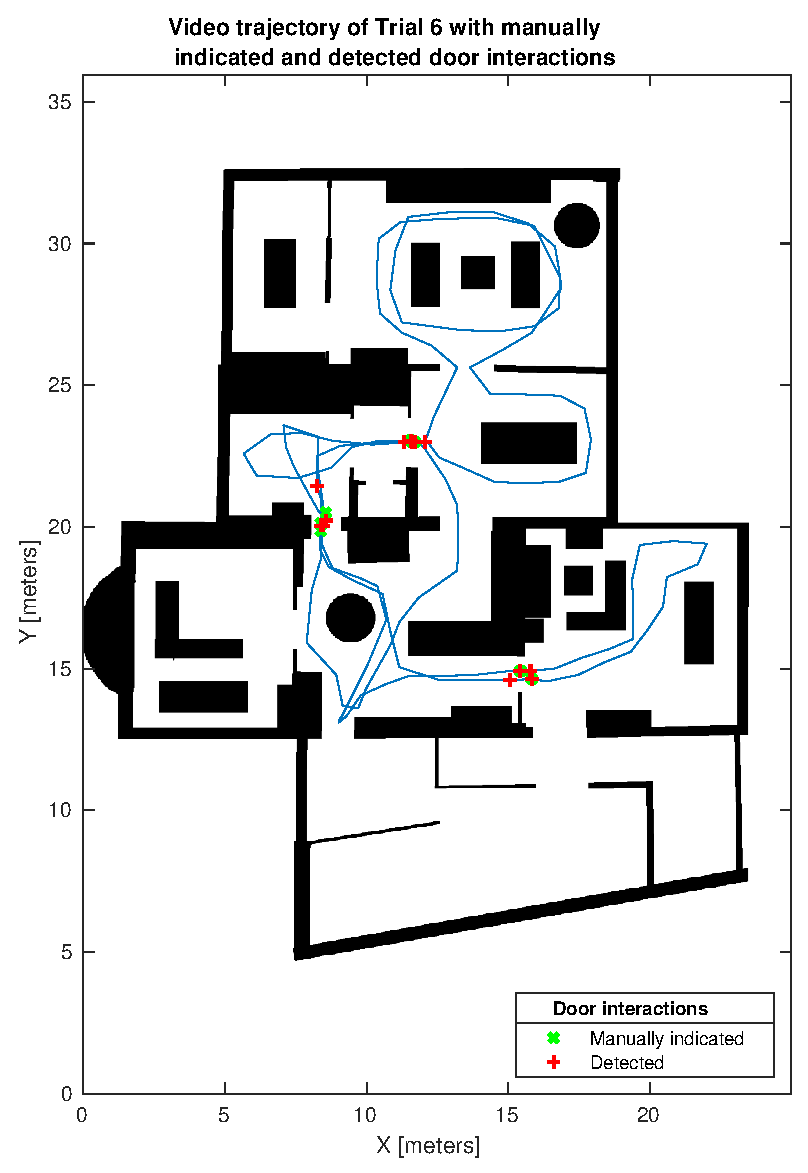
\includegraphics[width=0.7\linewidth]{images/20201129_2332_video_traj_Trial_6_door_detect_vs_manual_1}
	\setlength{\belowcaptionskip}{-20pt}
	\caption{Video trajectory for trial 6 with markers indicating position at time points when door interactions are either indicated manually or detected.}
	\label{fig:202011292332videotrajtrial6doordetectvsmanual1}
\end{figure}

\chapter{Extended Future Work List}
\label{chap:app-extended_future_work}
The following appendix chapter elaborates on the future research directions given within the thesis. For completeness the points in the thesis are listed as well. Within this chapter the different subsystem and their components will be treated through this perspective.

\subsection*{Step and Heading System }

The different components of the step and heading system subsystem have generated results with varying success. First the components are discussed, whereafter a closer look is taken of the whole subsystem.

\subsubsection*{Step Detection}

The step detection method outlined in \cref{sec:meth - step detection} has proven to work well for different carrying modes, with many carrying modes having a detection error around 5\% or less. One limitation of the method is that it was tested in environment in which the test subject were only walking around, not performing any other tasks. Testing how well it works with more complex movement will give more insight into the robustness of the approach. Movements typical of being performed in a residential setting could be considered.

\subsubsection*{Step Length Estimation}

Step length estimation using the step detection method outlined in thesis has shown different results than what was found in literature. No conclusive result could be made whether the accelerometer or frequency based method worked better, with performance of the approaches changing per test subject when applied to the opensource data of \citet{Vezocnik2019}. From experimental data, the performance of the approaches suggested that walking speed determined which worked best. The frequency based approach was chosen, with the reasoning that walking indoors was generally in the range of normal speed to slow speed, speeds with which this approach seemed to work best. \par 

Further research could focus on determining whether any of the other methods from \cite{Vezocnik2019} are able to estimate step length better when using the thesis step detection implementation of \cref{sec:meth - step detection}. The observation made that the models used do not seem to correspond well with the data used for parameter estimation could also be investigated further. More research can be done on techniques that apply similar offsets as introduced in \cref{sec:results-step_length-validation}. \par 

Another research direction worth considering is quantifying the effect that turning has on the step length, since all step length testing so far has been done while walking in a straight line. In addition, step length estimation in different carrying modes is a logical next step in increasing the applicability of the system in realistic situations. \par

The dataset of \citet{Bayev2019} can potentially help with improving step length estimation. The very large dataset contains data from smartphones carried in different carrying modes for over 60 people. It also has a ground truth estimate based off of a foot based INS-ZUPT method, as introduced in \cref{sec:rw-INS}. The combination allows for accurate step length measurements through INS-ZUPT, providing more measurement resolution that \cite{Vezocnik2019}. The size of the set provides opportunities for not only classical approaches as within this thesis, but more complex machine learning algorithms.\par

\subsubsection{Heading Estimation}

By simplifying heading estimation by only considering one carrying mode, the yaw Euler angle of the EKF orientation estimation of \cref{sec:meth-indoor_heading_estimation} represented the step heading within the Step and Heading System. Within this implementation, thresholds were used to adhere to the assumptions made by the orientation motion model used in the filter. \par 

One limitation within this thesis is that no quantitative comparison could be made to determine the orientation estimation performance. Only a comparison between orientation estimate of the Android system could be performed. Within the trials performed within the indoor experiments, trial 6 showed a large mean yaw difference with the Android system. Upon further inspection, the orientation estimation has a large spike close to the beginning of the trial. It is unclear what is causing this, and will need to be investigated further. Although faulty, this spike does not seem to effect the performance of position estimate. Using the orientation estimate of the android system for the step heading with the SHS did not position estimation by the particle filter. The particle filter was unable to complete any runs successfully. \par 

In general more experimentation is required to determine the performance of the heading estimation implementation used in this thesis. This could be done by performing the indoor experiments in combination with a higher quality \ac{IMU}, such as those produced by Xsens. A comparison can then be made between the orientation estimate of the Xsens device and the EKF implementation of \cref{sec:meth-indoor_heading_estimation}.\par 

The current heading estimation implementation can be enhanced to use different carrying modes, instead of just one. This would require implementing one of or a combination of the methods outlined in \cref{sec:rw-step_heading_estimation}. It would be interesting to see if the unconstrained methods are viable when taking spatial context into account.


\subsubsection{Overall Step and Heading Subsystem }

In \cref{sec:results-SHS_trajectories} a qualitative approach is used to give an indication of SHS performance with respect to the video position estimate. Further investigating this and generating a qualitative measure to compare performance could give more insight in to the criteria that an SHS trajectory must meet in order to lead to successful SHS-PF runs.

\subsection*{Particle Filter}
The particle filter uses spatial context to propagate position estimates. It does this by taking spatial constraints into account while estimating positions and performing a measurement update if a door interaction is detected or indicated manually. The movement of the estimates, called particles, is defined by a motion model based on the output of the SHS subsystem. The eventual position estimate of the particle filter is by calculating the trajectory of the particles at the last time step of the SHS, by determining the ancestor particles. These trajectories are averaged.

One aspect that was not for seen was that the method with which the position trajectory is determined within the Particle Filter is that it suffers from path degeneracy, where all particles share a common ancestor \cite{Lindsten2013}. A method such as Forward Filter - Backward Smoothing is worth considering \cite{Lindsten2013}.

Another approach is to use a Back Tracking Particle Filter (BTFP) . The BTPF takes particles that are not valid at some time step $ k $ and calculates the particle trajectories that lead to those particles up to some point $ k - n $, where n is set beforehand. The state estimates at time k-n are then recalculated without the removed particles using for example RMSE or MAP. Each particle has to remember its state history or trajectory to facilitate backtracking. 

More research in the effect of different particle numbers is also a direction worth considering.

\subsection{Door Interaction Activity Recognition}

The door interaction measurement update performed by the spatial context Particle Filter compares particle positions to the closest door if an interaction is detected, changing their weights accordingly. The door interaction detection method used in this thesis uses thresholds on the accelerometer data from a smartwatch in combination with standstill detection based on step detection of the \ac{SHS}. The smartwatch was placed on the wrist of the hand that interacted with the doors during the experiments.\par 

The scope of this thesis was not to create the best activity recognition implementation. However, the experiments indicated that the door interaction detection method, although relatively simple, was effective at detecting door interactions. Only one false positive was observed throughout all 6 trials. \par 

During the indoor experiments, the hand with the smartwatch was only used to open doors. The door detection implementation would need to be tested for robustness against other activities performed with the smartwatch hand, to get a further indication of performance in a realistic setting. \par 

Activity recognition through smartwatch IMU data could also be enhanced to detect other position dependent activities, which could be used to trigger measurement updates within the spatial context Particle Filter. The same could be  done with the combination of smartphone and smartwatch IMU data, a combination that has been shown to improve activity recognition \cite{Shoaib2016}.

\subsection{Indoor Experiment Setup}

The experiments performed to test the complete SHS-PF indoor localization system were performed in a residential building, while filming the trials from a breast pocket. In post processing the videos per trial were replayed and used to manually indicate the position of the test subject over time within the indoor environment. This manually generated trajectory within the indoor environment was used to determine performance of the SHS-PF. \par 

An improvement that can be made for this experimental setup is a more accurate ground truth estimate. A test environment in which the infrastructure dependent solutions can be leveraged could potentially generate a viable solution. Additional research would be required to determine if visual odometry can produce another possibility. \par

An interesting research direction worth considering is testing the current implementation in different types of buildings. It has currently been tested in a residential building, in which there are no clear walking paths. In larger buildings with a more corridor style indoor environment, the position estimates of the Particle Filter could be more restricted, therefore having better position estimation.
